%
%   $Id$
%   This file is part of the FPC documentation.
%   Copyright (C) 2000 by Florian Klaempfl
%
%   The FPC documentation is free text; you can redistribute it and/or
%   modify it under the terms of the GNU Library General Public License as
%   published by the Free Software Foundation; either version 2 of the
%   License, or (at your option) any later version.
%
%   The FPC Documentation is distributed in the hope that it will be useful,
%   but WITHOUT ANY WARRANTY; without even the implied warranty of
%   MERCHANTABILITY or FITNESS FOR A PARTICULAR PURPOSE.  See the GNU
%   Library General Public License for more details.
%
%   You should have received a copy of the GNU Library General Public
%   License along with the FPC documentation; see the file COPYING.LIB.  If not,
%   write to the Free Software Foundation, Inc., 59 Temple Place - Suite 330,
%   Boston, MA 02111-1307, USA.
%
%%%%%%%%%%%%%%%%%%%%%%%%%%%%%%%%%%%%%%%%%%%%%%%%%%%%%%%%%%%%%%%%%%%%%
% The IDE
%%%%%%%%%%%%%%%%%%%%%%%%%%%%%%%%%%%%%%%%%%%%%%%%%%%%%%%%%%%%%%%%%%%%%
\chapter{The IDE}

The IDE (\textbf{I}ntegrated \textbf{D}evelopment \textbf{E}nvironment)
provides a comfortable user interface to the compiler. It contains an 
editor with syntax highlighting, a debugger, symbol browser etc. 
The IDE is a textmode application which has the same look and feel 
on all supported operating systems. It is modeled after the IDE of Turbo
Pascal, so many people should feel comfortable using it.

Currently, the IDE is available for \dos, \windows and \linux.

%%%%%%%%%%%%%%%%%%%%%%%%%%%%%%%%%%%%%%%%%%%%%%%%%%%%%%%%%%%%%%%%%%%%%%%
% First steps with the IDE
\section{First steps with the IDE}
%
% Starting the IDE
%
\subsection{Starting the IDE}
The IDE is started by entering the command:
\begin{verbatim}
fp
\end{verbatim}
at the command line. It can also be started from a graphical user 
interface such as \windows. 
\begin{remark}
Under \windows, it is possible to switch between windowed mode and 
full screen mode by pressing \key{Alt-Enter}).
\end{remark}
%
% IDE command-line options.
%
\subsection{IDE Command line options}
When starting the IDE, command line options can be passed:
\begin{verbatim}
fp [-option] [-option] ... <file name> ...
\end{verbatim}
\var{Option} is one of the following switches (the option letters
are case insensitive):
\begin{description}
\item [-N] (\dos only) Do not use long file names. \windows 95 and later
versions of \windows provide an interface to DOS applications to access 
long file names. 
The IDE uses this interface by default to access files. Under certain 
circumstances, this can lead to problems. This switch tells the IDE not to
use the long filenames.
\item [-Cfilename] This option, followed by a filename, tells the IDE to
read its options from \file{filename}. There should be no whitespace between
the file name and the \var{-C}.
\item [-F] use alternative graphic characters. This can be used to run the
IDE on \linux in an X-term or through a telnet session.
\item [-R] After starting the IDE, it changes automatically to the directory
which was active when the IDE exited the last time.
\item [-S] Disable the mouse. When this option is used, then the mouse is
disabled, even if a mouse is present.
\end{description}
The files given at the command line are loaded into edit windows automatically.

\begin{remark}
Under DOS/Win32, a \var{/} can be used instead of \var{-} to pass a
command line switch to the IDE.
\end{remark}

\subsection{The IDE screen}

After start up, the screen of the IDE can look like 
\begin{htmlonly}
this:
\htmladdimg{../pics/idestart.gif}
\end{htmlonly}
\begin{latexonly}
\seefig{idestart}.
\begin{figure}
\caption{The IDE screen immediatly after startup}
\label{fig:idestart}
\ifpdf
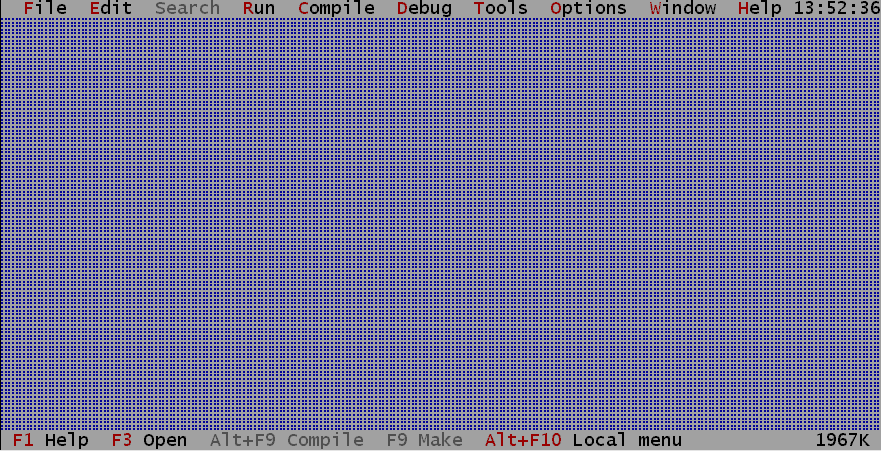
\epsfig{file=pics/idestart.png,width=\textwidth}
\else
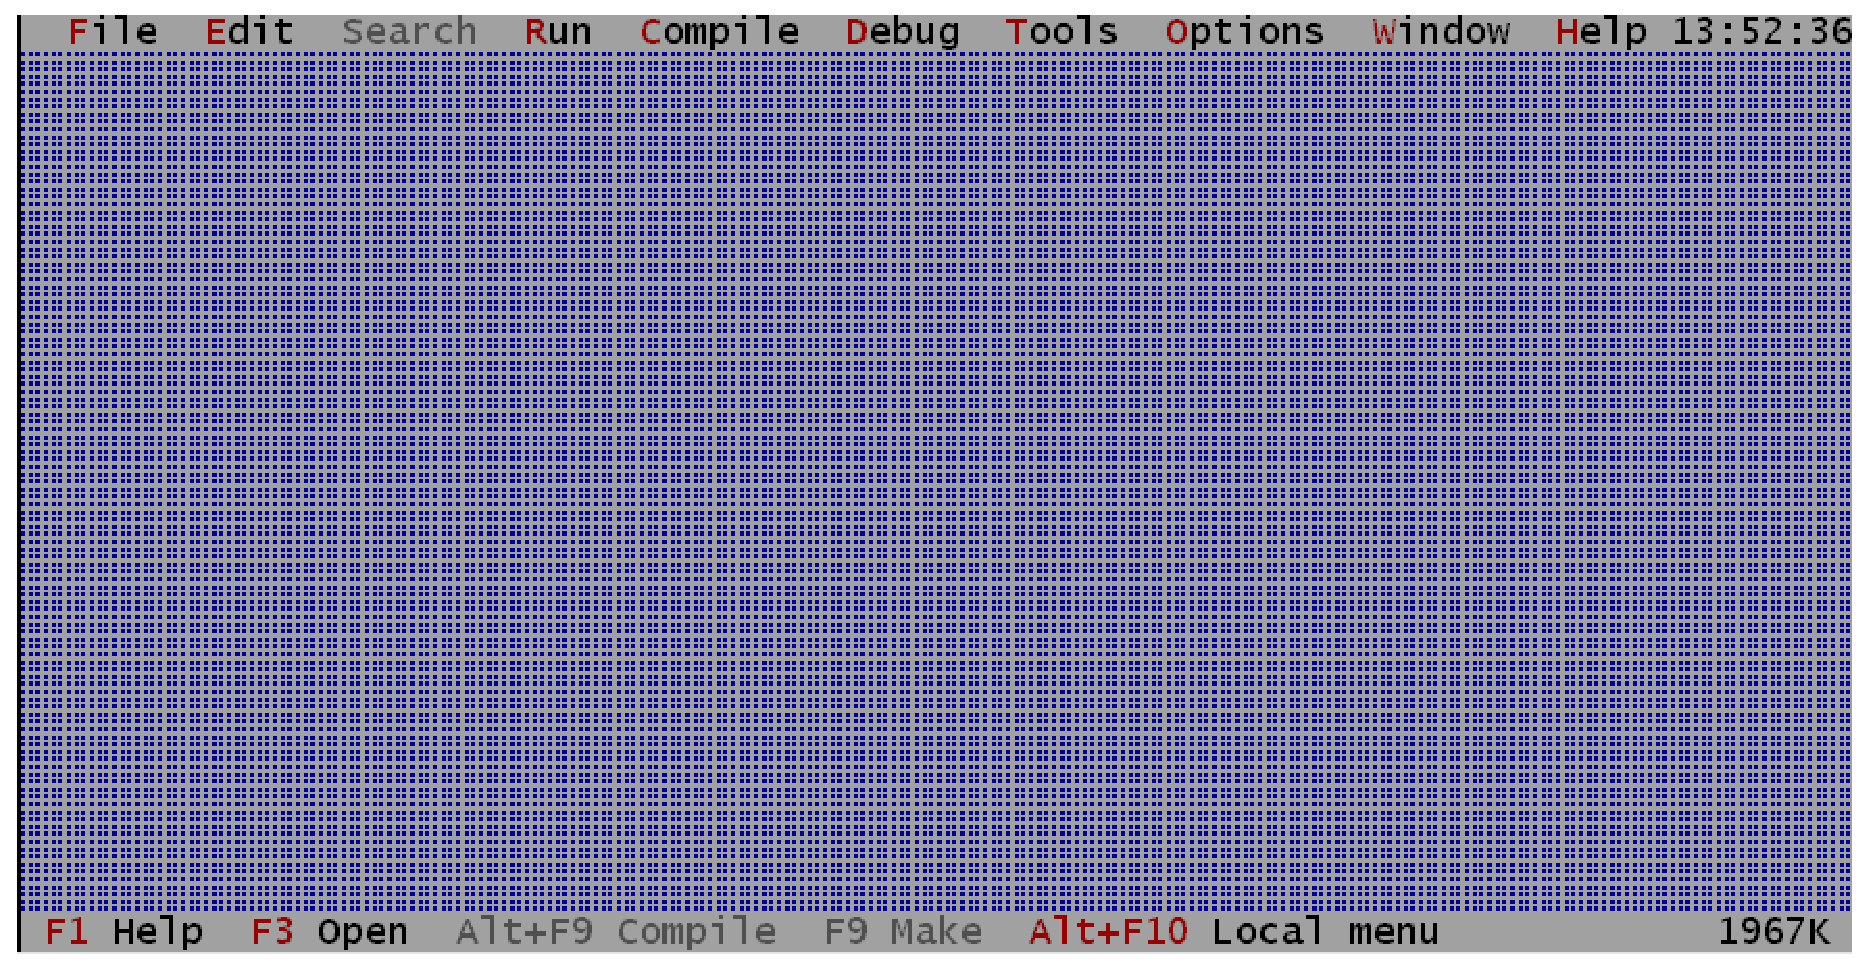
\epsfig{file=pics/idestart.eps,width=\textwidth}
\fi
\end{figure}
\end{latexonly}
At top of the screen the \emph{menu bar} is visible, at the bottom
the \emph{status bar}. The empty space between them is called the
\emph{desktop}.

The statusbar shows the keyboard shortcuts for frequently used 
commands, and allows quick access to these commands by clicking 
them with the mouse. 
At the right edge of the statusbar, the current amount of unused 
memory is displayed. This is only an indication, since the IDE 
tries to allocate more memory from the operating system if it 
runs out of memory.

The menu provides access to all of the IDE's functionality, and
at the right edge of the menu, a clock is displayed.

The IDE can be left by selecting \menu{File|Exit} in the menu
\footnote{\menu{File|Exit} means select the item 'Exit' in the menu 'File'.}
or by pressing \key{Alt-X}.

\begin{remark}
If a file \file{fp.ans} is found in the current directory,
then it is loaded and used to paint the background.
This file should contain ANSI drawing commands to draw on a screen.
\end{remark}

%%%%%%%%%%%%%%%%%%%%%%%%%%%%%%%%%%%%%%%%%%%%%%%%%%%%%%%%%%%%%%%%%%%%%%%
% Navigating in the IDE
\section{Navigating in the IDE}
The IDE can be navigated both with the keyboard and with a mouse, if your
system has a mouse.
%
% Using the keyboard
%
\subsection{Using the keyboard} 
All functionality of the IDE is available through use of the keyboard.
\begin{itemize}
\item It is used for typing and navigating through the sources.
\item Editing commands such as copying and pasting text.
\item Moving and resizing windows.
\item It can be used to access the menu, by pressing \key{ALT} and the
appropriate highlighted menu letter, or by pressing \key{F10} and
navigating through the menu with the arrow keys.

more information on the menu can be found in \sees{idemenu}
\item Many commands in the IDE are bound to shortcuts, i.e. typing a special
combination of keys will execute a command immediatly.
\end{itemize}
\begin{remark}
\begin{itemize}
\item When working in a \linux X-Term or through a telnet session, the
keycombination with \key{Alt} may not be available. To remedy this, the 
\key{Ctrl-Z} combination can be typed first. This means that e.g. \key{Alt-X}
can be replaced by \key{Ctrl-Z X}.
\item A complete reference of all keyboard shortcuts can be found in
\sees{keyshortcuts}.
\end{itemize}
\end{remark}
% 
% Using the mouse
%
\subsection{Using the mouse}
\label{suse:mouseusage}
If the system is equipped with a mouse, it can be used to work with the
IDE. The left button is used to select menu items, press buttons, select
text blocks etc. 

The right mouse button is used to access the local menu, if
it is available. Holding down the \key{Ctrl} or \key{Alt} key and 
clicking the right button will execute user defined functions, 
see \sees{prefmouse}.

\begin{remark}
\begin{enumerate}
\item Occasionally, the manual uses the term "drag the mouse". This
means that the mouse is moved while the left mouse button is being 
pressed.
\item 
The action of mouse buttens may be reversed, i.e. the actions of the left
mouse button can be assigned to the right mouse button and vice versa  
\footnote{See \sees{prefmouse} for more information on how to reverse the
actions of the mouse buttons.}. Throughout the manual, it is assumed 
that the actions of the mouse buttons are not reversed.
\item
The mouse is not allways available, even if a mouse is installed:
\begin{itemize}
\item The IDE is running under \linux throught a telnet connection from 
a \windows machine.
\item The IDE is running under \linux in an X-term under X-windows.
\end{itemize}
\end{enumerate}
\end{remark}
%
% Navigating in dialogs
% 
\subsection{Navigating in dialogs}
\label{se:navigatingdialogs}
Dialogs usually have a lot of elements in them such as buttons, edit fields,
memo fields, list boxes and so on. To activate one of these fields, it is
sufficient to:
\begin{enumerate}
\item Click on the element with the mouse.
\item Press the \key{Tab} key till the focus reaches the mouse
\item Press the highlighted letter in the element's label. If the focus
is currently on an element that allows to edit, then \key{Alt} should be
pressed simultaneously with the highlighted letter. For a button, the action
asociated with the button will then be executed.
\end{enumerate}
Inside edit fields, list boxes, memos, navigation is carried out with the
usual arrow key commands.

%%%%%%%%%%%%%%%%%%%%%%%%%%%%%%%%%%%%%%%%%%%%%%%%%%%%%%%%%%%%%%%%%%%%%%%
% Windows
\section{Windows}
\label{se:windows}
Nowadays, working with windowed applications should be no problem for
most \windows and \linux users. Nevertheless, the following section 
describes how the windows work in the \fpc IDE, to allow efficient 
work with it.
%
% Window basics
%
\subsection{Window basics}
\label{se:windowbasics}
\begin{htmlonly}
A common IDE window is displayed  below:
\htmladdimg{../pics/idewin.gif}
\end{htmlonly}
\begin{latexonly}
A common IDE window is displayed in \seefig{idewin}.
\begin{figure}
\caption{A common IDE window}
\label{fig:idewin}
\ifpdf
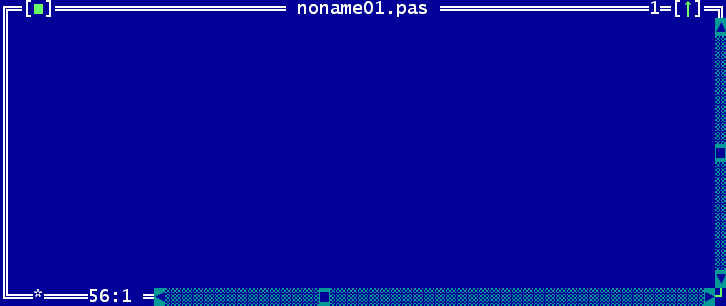
\epsfig{file=pics/idewin.png,width=\textwidth}
\else
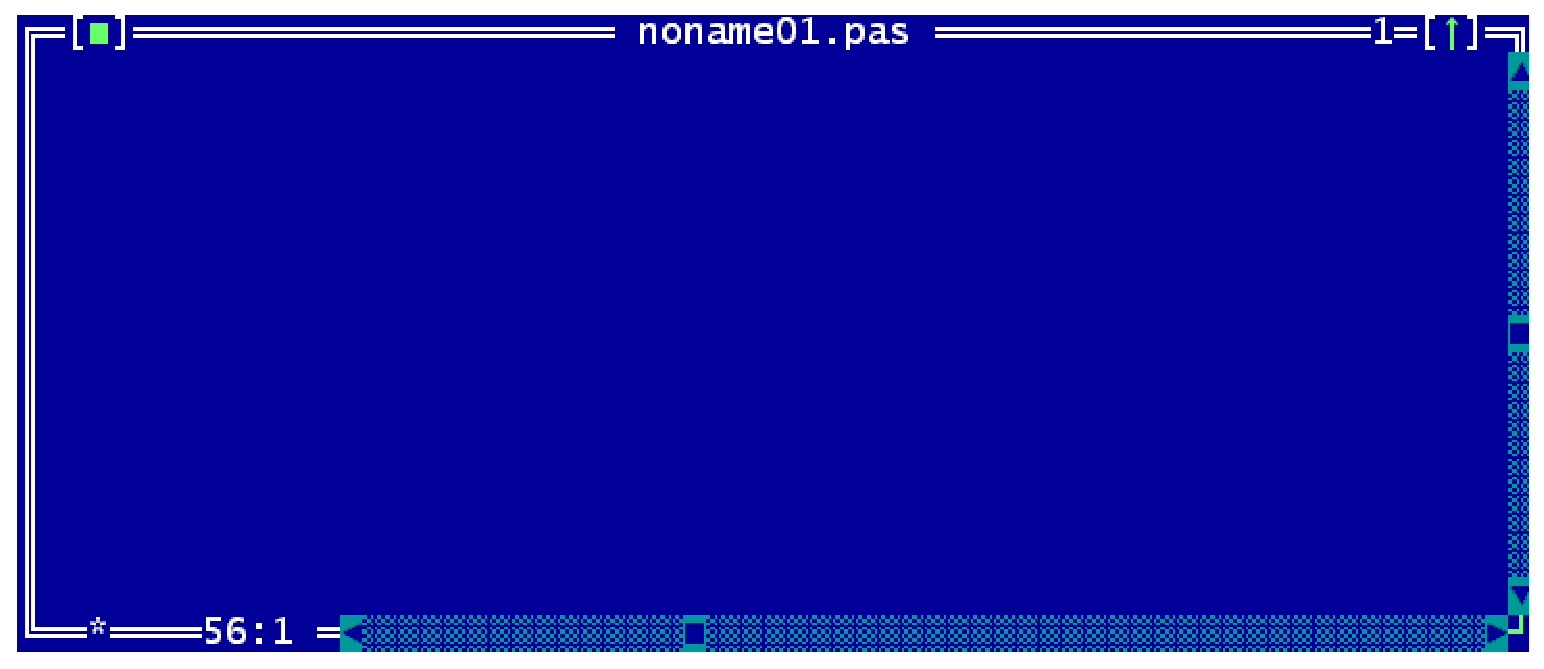
\epsfig{file=pics/idewin.eps,width=\textwidth}
\fi
\end{figure}
\end{latexonly}
The window is surrounded by a so-called \emph{frame}, the white double
line around the window. 

At the top of the window 4 things are displayed:
\begin{itemize}
\item 
At the upper left corner of the window, a \emph{close icon} is shown. 
When clicked, the window will be closed. It can be also closed by
 pressing \key{Alt-F3} or selecting the menu item \menu{Window|Close}. 
All open windows can be closed by selecting the menu item 
\menu{Window|Close all}.
\item In the middle, the title of the window is displayed.
\item Almost at the upper right corner, a number is visible.
This number identifies the editor window, and pressing \key{Alt-Number}
will jump to this window. Only the first 9 windows will get such a number.
\item At the upper right corner, a small green arrow is visible.
Clicking this arrow zooms the window so it covers the whole desktop. 
Clicking this arrow on a zoomed window will restore old size of the 
window. Pressing the key \key{F5} has the same effect as clicking 
that arrow. The same effect can be achieved with the menu item 
\menu{Window|Zoom}. 
Windows and dialogs which aren't resizeable can't be zoomed, either.
\end{itemize}

The right edge and bottom edges of a window contain scrollbars.
They can be used to scroll the window contents with the mouse. 
The arrows at the ends of the scrollbars can be clicked to scroll the 
contents line by line. Clicking on the dotted area between the arrows 
and the cyan-coloured rectangle will scroll the window's content 
page by page. By dragging the rectangle the content can be scrolled 
continuously.

The star and the numbers in the lower left corner of the window
display information about the contents of the window. They
are explained in the section about the editor, see \sees{editingtext}.

%
% Sizing+moving windows
%
\subsection{Sizing and moving windows}
\label{se:windowsizingmoving}
A window can be moved and sized using the mouse and the keyboard:
To move a window, either:
\begin{itemize}
\item using the mouse, click on the title bar and drag the window 
with the mouse.
\item using the keyboard, go into the size/move mode
by pressing \key{Ctrl-F5} or selecting the menu item
\menu{Window|Size/Move}. . Using the cursor keys the window can be moved. 
The size/move mode can be left by pressing \key{Enter}. 
In this case, the window will keep its size and position. 
Alternativly, pressing \key{Esc} will restore the old position.
\end{itemize} 
To resize a window, either:
\begin{itemize}
\item using the mouse, click on the lower right corner of the window
and drag it.
\item using the keyboard, go into the size/move mode
by pressing \key{Ctrl-F5} or selecting the menu item
\menu{Window|Size/Move}. The window frame will be green to indicate that
the IDE is in size/move mode. 
By pressing shift and the cursor keys simultaneously, the window can 
be resized.  The size/move mode can be left by pressing
\key{Enter}. In this case, the window will keep the new size.
Pressing \key{Esc} will restore the old size.
\end{itemize}
Not all windows can be resized. This applies, for example, to
\emph{dialog windows} (\sees{dialogwindow}).

A window can also be hidden. To hide a window, the \key{Ctrl-F6} key
combination can be used, or the \menu{Window|Hide} menu may be selected.
To restore a Hidden window, it is necessary to select it from the window
list. More information about the window list can be found in the next
section.   
%
% Multiple windows
%
\subsection{Working with multiple windows}
\label{se:multiplewindows}
When working with larger projects, it is likely that multiple windows 
will appear on the desktop. However, only one of these windows will be 
the active window, all other windows will be inactive.

An inactive window is identified by a grey frame. An inactive window can
be made active in one of several ways:
\begin{itemize}
\item using the mouse, activate a window by clicking on it.
\item using the keyboard, pressing \key{F6} will step trough all open 
windows. To activate the previously activated window, \key{Shift-F6} can
be used.
\item the menu item \menu{Window|Next} can be used to activate the next 
window in the list of windows, while \var{Window|Previous} will select
the previous window.
\item If the window has a number in the upper right corner, it can be
activated by pressing \key{Alt-<number>}.
\item Pressing \key{Alt-0} will pop up a dialog with all 
available windows which allows a quick activation of windows which 
don't have a number.
\end{itemize}

The windows can be ordered and placed on the IDE desktop by zooming and
resizing them with the mouse or keyboard. This is a time-consuming task, 
and particularly difficult with the keyboard. Instead, the menu items
\menu{Window|Tile} and \menu{Window|Cascade} can be used:
\begin{description}
\item[Tile] will divide whole desktop space evenly between all resizable 
windows. 
\item[Cascade] puts all windows in a cascaded position. 
\end{description}

In very rare cases the screen of the IDE may be mixed up. In this
case the whole IDE screen can be refreshed by selecting the menu item 
\menu{Window|Refresh display}.
%
% Dialog windows
%
\subsection{Dialog windows}
\label{se:dialogwindow}
In many cases the IDE displays a dialog window to get user input.
The main difference to normal windows is that other windows cannot be
activated while a dialog is active. Also the menu is not accessible while in
a dialog. This behavior is called \emph{modal}. To activate another window, 
the modal window or dialog must be closed first.

\begin{htmlonly}
A typical dialog window looks like:
\htmladdimg{../pics/idedlg.gif}
\end{htmlonly}
\begin{latexonly}
A typical dialog window is shown in \seefig{idedlg}.
\begin{figure}
\caption{A typical dialog window}
\label{fig:idedlg}
\ifpdf
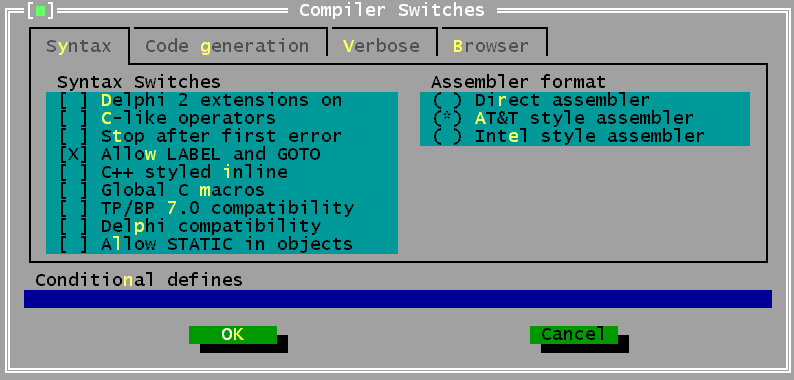
\epsfig{file=pics/idedlg.png,width=\textwidth}
\else
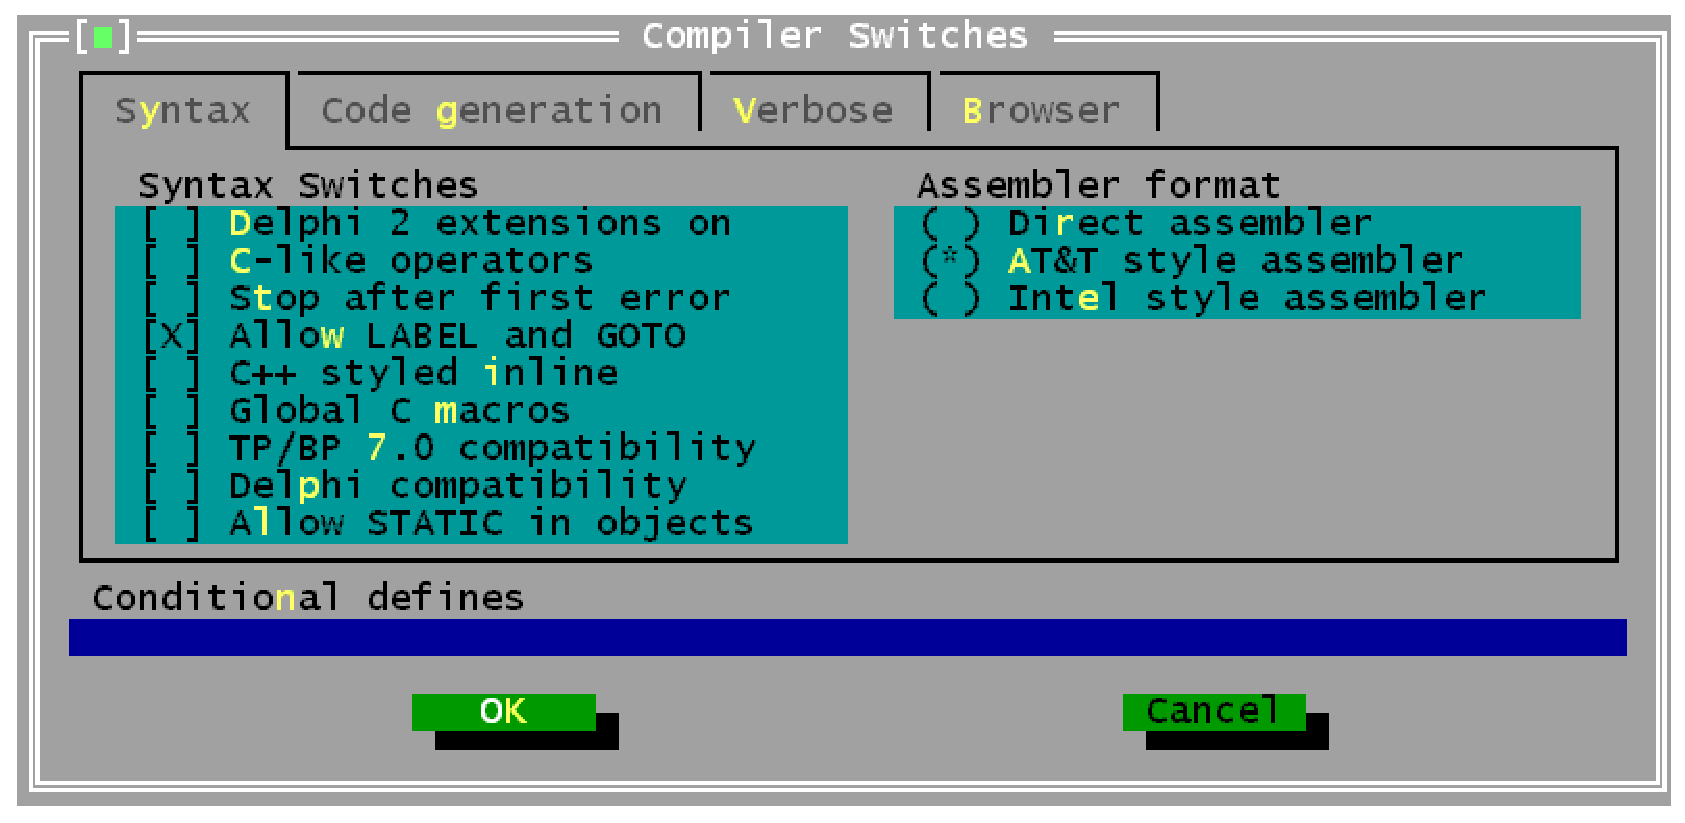
\epsfig{file=pics/idedlg.eps,width=\textwidth}
\fi
\end{figure}
\end{latexonly}

%%%%%%%%%%%%%%%%%%%%%%%%%%%%%%%%%%%%%%%%%%%%%%%%%%%%%%%%%%%%%%%%%%%%%%%
% The menu
\section{The Menu}
\label{se:idemenu}
The main menu (the gray bar at the top of the IDE) provides access to all the
functionality of the IDE. It also displays a clock, displaying the current
time. The menu is always available, except when a dialog is opened. If a
dialog is opened, it must be closed first in order to access the menu.

In certain windows, a local menu is also available. The local menu will
appear where the cursor is, and provides additional commands that are 
context-sensitive.
%
% Accessing the menu
%
\subsection{Accessing the menu}
The menu can be accessed in a number of ways:
\begin{enumerate}
\item By using the mouse to select items. The mouse cursor should be located
over the desired menu item, and a left mouse click will then select it.
\item By pressing \key{F10}. This will switch the IDE focus to the menu. 
Use the arrow keys can then be used to navigate in the menu, the 
\key{Enter} key should be used to select items.
\item To access menu items directly, \key{Alt-<highlighted menu letter>}
can be used to select a menu item. Afterwards submenu entries can be selected 
by pressing the highlighted letter, but without \key{Alt}. 
E.g. \key{Alt-S G} is a fast way to display the \emph{goto line} dialog.
\end{enumerate}
Every menu item is explained by a short text in the status bar.

When a local menu is available, it can be accessed by pressing
the right mouse button or \key{Alt-F10}. 

In the subsequent, all menu entries and their actions are described.
%
% The file menu
%
\subsection{The File menu}
\label{se:menufile}
The \menu{File} menu contains all menu items that allow to load and save file, as
well as to exit the IDE.
\begin{description}
\item[New] Opens a new, empty editor window. 
\item[New from template] Prompts for a template to be used, asks to fill in
any parameters, and then starts a new editor window with the template.
\item[Open] (\key{F3}) Presents a file selection dialog, and opens 
the selected file in a new editor window. 
\item[Save] (\key{F2}) Saves the contents of the current edit window 
with the current filename. If the current edit window does not yet have
a filename, a dialog is presented to enter a filename.
\item[Save as] Presents a dialog in which a filename can be entered. The
current window's contents are then saved to this new filename, and the
filename is stored for further save actions.
\item[Change dir] Presents a dialog in which a directory can be selected.
The current working directory is then changed to the selected directory.
\item[Dos shell] Executes a command shell. After the shell exited, the
IDE resumes.
\item[Exit] (\key{ALT-X}) Exits the IDE. If any unsaved files are 
in the editor, the IDE will ask if these files should be saved.
\end{description}
Under the \menu{Exit} menu appear some filenames of recently used files.
These entries can be used to quickly reload these files in the editor.

%
% The edit menu
%
\subsection{The Edit menu}
\label{se:menuedit}
The \menu{Edit} menu contains entries for accessing the clipboard, and
undoing or redoing editing actions. Most of these functions have shortcut
keys associated with them.
\begin{description}
\item[Undo] (\key{ALT-BKSP})
Undo the last editing action. The editing actions are stored in a buffer,
selecting this mechanism will move backwards through this buffer, i.e.
multiple undo levels are possible. The selection is not preserved, though.
\item[Redo] Redo the last action that was previously undone. Redo can redo
multiple undone actions. 
%\item[Dump undo]
%Shows the contents of the UNDO list in the messages window.
%\item[Undo all]
%Undo all actions in the undo buffer. If a new empty file was started, this
%action should clear the window contents again.
%\item[Redo all]
%Redo all editing actions that were undone.
\item[Cut] (\key{Shift-DEL}) Copy the current selection to the clipboard
and delete the selection from the text. Any previous clipboard contents is
lost after this action. After this action, the clipboard contents can be 
pasted elsewhere in the text.
\item[Copy] (\key{Ctrl-INS}) Copy the current selection to the clipboard.
Any previous clipboard contents is lost after this action. 
After this action, the clipboard contents can be pasted elsewhere in the text.
\item[Paste] (\key{Shift-INS}) Insert the current clipboard contents in
the text at the cursor position. The clipboard contents remains as it was.
\item[Clear] (\key{Ctrl-DEL}) Clears (i.e. deletes) the current
selection.
\item[Show clipboard] Opens a window in which the current clipboard contents
is shown.
\end{description}
When running an IDE under \windows, the \menu{Edit} menu has two
additional entries. The IDE maintains a separate clipboard which does 
not share its contents with the windows clipboard. To access the Windows
clipboard, the following two entries are also present:
\begin{description}
\item[Copy to Windows] this will copy the selection to the Windows
clipboard. 
\item[Paster from windows] this will insert the content of the windows
clipboard (if it contains text) in the edit window at the current cursor
position.
\end{description}

%
% The Search menu
%
\subsection{The Search menu}
\label{se:menusearch}
The \menu{Search} menu provides acces to the search and replace dialogs, as well as
access to the symbol browser of the IDE. 
\begin{description}
\item[Find] (\key{Ctrl-Q F}) Presents the search dialog. A search text 
can be entered, and when the dialog is closed, the entered text is searched
in the active window. If the text is found, it will be selected. 
\item[Replace] (\key{Ctrl-Q A}) Presents the search and replace dialog.
After the dialog is closed, the search text will be replaced by the replace
text in the active window.
\item[Search again] (\key{CTRL-L}) Repeats the last search or search and replace action,
 using  the same parameters.
\item[Go to line number] (\key{Alt-G}) Prompts for a line number, and
then jumps to this line number.
\end{description}
When the program and units are compiled with browse information, then
the following menu entries are also enabled:
\begin{description}
\item[Find procedure]
Not yet implemented.
\item[Objects]
Asks for the name of an object and opens a browse window for this object.
\item[Modules]
Asks for the name of a module and opens a browse window for this object.
\item[Globals]
Asks for the name of a global symbol and opens a browse window for this object.
\item[Symbol]
Opens a window with all known symbols, so a symbol can be selected. After
the symbol is selected, a browse window for that symbol is opened.
\end{description}
%
% The Run menu
%
\subsection{The Run menu}
\label{se:menurun}
The \menu{Run} menu contains all entries related to running a program,
\begin{description}
\item[Run] (\key{Ctrl-F9})
If the sources were modified, compiles the program. If the compile is
successful, the program is executed. If the primary file  was set, then 
that is used to determine which program to execute. See \sees{menucompile}
for more information on how to set the primary file.
\item[Step over] (\key{F8})
Run the program till the next source line is reached. If any calls to 
procedures are made, these will be executed completely as well.
\item[Trace into] (\key{F7})
Execute the current line. If the current line contains a call to another
procedure, the process will stop at the entry point of the called procedure.
\item[Goto cursor] (\key{F4})
Runs the program till the execution point matches the line where the cursor
is.
\item[Until return]
Runs the current procedure till it exits.
\item[Parameters]
This menu item allows to enter parameters that will be passed on to the
program when it is being executed.
\item[Program reset] (\key{Ctrl-F2}) if the program is being run or 
debugged, the debug session is aborted, and the running program is killed.
\end{description}
%
% The compile menu
%
\subsection{The Compile menu}
\label{se:menucompile}
The \menu{Compile} menu contains all entries related to compiling a program or
unit.
\begin{description}
\item[Compile] (\key{Alt-F9}) Compiles the contents of the active window,
irrespective of the primary file setting.
\item[Make] (\key{F9}) Compiles the contents of the active window, and
any files that the unit or program depends on and that were modified since
the last compile.
If the primary file was set, the primary file is compiled instead.
\item[Build]
Compiles the contents of the active window, and any files that the unit or 
program depends on, whether they were modified or not.
If the primary file was set, the primary file is compiled instead.
\item[Target] Sets the target operating system for which should be compiled. 
\item[Primary file] Sets the primary file. If set, any run or compile command 
will act on the primary file instead of on the active window. The primary
file need not be loaded in the IDE for this to have effect.
\item[Clear primary file]
Clears the primary file. After this command, any run or compile action will
act on the active window.
\item[Information] Displays some information about the current program.
\item[Compiler messages] (\key{F12}) Displays the compiler messages
window. This window will display the messages generated by the compiler
during the last compile.
\end{description}
%
% The debug menu
%
\subsection{The Debug menu}
\label{se:menudebug}
The \menu{Debug} menu contains menu entries to aid in debugging a program, such as
setting breakpoints and watches. 
\begin{description}
\item[Output]
\item[User screen] (\key{Alt-F5})
Switches to the screen as it was last left by the running program.
\item[Breakpoint] (\key{Ctrl-F8})
Sets a breakpoint at the current line. When debugging, program execution
will stop at this breakpoint.
\item[Call stack] (\key{Ctrl-F3})
Shows the call stack. The call stack is the list of addresses (and
filenames and line numbers, if this information was compiled in) of 
procedures that are currently being called in the running program.
\item[Registers]
Shows the current content of the CPU registers. 
\item[Add watch] (\key{Ctrl-F7}) Add a watch. A watch is an expression
that can be evaluated by the IDE and shown in a special window. usually this
is the contents of some variable. 
\item[Watches]
Shows the current list of watches in a separate window.
\item[Breakpoint list]
Shows the current list of breakpoints in a separate window.
\item[GDB window]
Shows the GDB debugger console. This can be used to interact with the debugger
directly.
\end{description}
%
% The tools menu
%
\subsection{The Tools menu}
\label{se:menutools}
The \menu{Tools} menu defines some standard tools. If new tools are defined by the
user, they are appended to this menu as well.
\begin{description}
\item[Messages] (\key{F11}) Show the messages window. 
This window contains the output from one of the tools. For more information,
see \sees{toolsmessages}.
\item[Goto next] (\key{Alt-F8}) Goto next message.
\item[Goto previous] (\key{Alt-F7}) Goto previous message
\item[Grep] (\key{SHIFT-F2}) Prompts for a regular expression and options
to be given to grep, and then executes \file{grep} with the given expression and
options. For this to work, the \file{grep} program must be installed on your
system, and be in a directory that is in the \var{PATH}. For more
information, see \sees{grep}.
\item[Calculator] 
Displays the calculator. For more information, see \sees{calculator}
\item[Ascii table] Displays the \var{ASCII} table. For more information, see
\sees{asciitable}
\end{description}
%
% The Options menu
%
\subsection{The Options menu}
\label{se:menuoptions}
The \menu{Options} menu is the entry point for all dialogs that are used to set
options for compiler and IDE, as well as the user preferences.
\begin{description}
\item[Mode] Presents a dialog to set the current mode of the compiler. The
current mode is shown at the right of the menu entry. For more information,
see \sees{compilermode}.
\item[Compiler] Presents a dialog that can be used to set common compiler
options. These options will be used when compiling a program or unit.
\item[Memory sizes]
Presents a dialog where the stack size and the heap size for the program can
be set. These options will be used when compiling a program.
\item[Linker]
Presents a dialog where some linker options can be set. These options will
be used when a program or library is compiled.
\item[Debugger]
Presents a dialog where the debugging options can be stored. These options
are used when compiling units or programs. Note that the debugger will not
work unless debugging information is generated in the program.
\item[Directories]
Presents a dialog where the various directories needed by the compiler can
be set. These directories will be used when a program or unit is compiled.
\item[Browser]
Presents a dialog where the browser options can be set. The browser options
affect the behaviour of the symbol browser of the IDE. 
\item[Tools]
Presents a dialog to configure the tools menu. For more information, see
\sees{addingtools}.
\item[Environment]
Presents a dialog to configure the behaviour of the IDE. A sub menu is
presented with the various aspects of the IDE:
\begin{description}
\item[Preferences]
General preferences, such as whether to save files or not, and which files
should be saved. The video mode can also be set here.
\item[Editor]
Controls various aspects of the edit windows.
\item[CodeComplete]
Used to set the words which can be automatically completed when typing in
the editor windows.
\item[Codetemplates]
Used to define code templates, which can be inserted in an edit window.
\item[Desktop]
Used to control the behaviour of the desktop, i.e. several features can be
switched on or off.
\item[Mouse]
Can be used to control the actions of the mouse, and to assign commands to
various mouse actions.
\item[Startup]
Not yet implemented.
\item[Colors]
Here the various colors used in the IDE and the editor windows can be set.
\end{description}
\item[Open]
Presents a dialog in which a file with editor preferences can be selected. 
after the dialog is closed, the preferences file will be read and the
preferences will be applied.
\item[Save]
Save the current options in the default file.
\item[Save as]
Saves the current options in an alternate file. A file selection dialog box
will be presented in which the alternate settings file can be entered.
\end{description}
Please note that options are not saved automatically, they should be saved
explicitly with the \menu{Options|\-Save} command.
%
% The window menu
%
\subsection{The Window menu}
\label{se:menuwindow}
The \menu{Window} menu provides access to some window functions. More information
on all these functions can be found in \sees{windows}
\begin{description}
\item[Tile]
Tiles all opened windows on the desktop.
\item[Cascade]
Cascades all opened windows on the desktop.
\item[Close all]
Close all opened windows.
\item[Size/move] (\key{Ctrl-F5})
Put the IDE in Size/move modus; after this command the active window can be
moved and resized using the arrow keys.
\item[Zoom] (\key{F5})
Zooms or unzooms the current window. 
\item[Next] (\key{F6})
Activates the next window in the window list.
\item[Previous] (\key{SHIFT-F6})
Activates the previous window in the window list.
\item[Hide] (\key{Ctrl-F6})
Hides the active window. 
\item[Close] (\key{ALT-F3})
Closes the active window.
\item[List] (\key{Alt-0})
Shows the list of opened windows. From there a
window can be activated, closed, shown and hidden.
\item[Refresh display]
Redraws the screen.
\end{description}
%
% The Help menu
%
\subsection{The Help menu}
\label{se:menuhelp}
The \menu{Help} menu provides entry points to all the help functionality of
the IDE, as well as the entry to customize the help system.
\begin{description}
\item[Contents]
Shows the help table of contents
\item[Index] (SHIFT-F1)
Jumps to the help Index.
\item[Topic search]  (CTRL-F1)
Jumps to the topic associated with the currently highlighted text.
\item[Previous topic] (ALT-F1)
Jumps to the previously visited topic.
\item[Using help]
Displays help on using the help system.
\item[Files]
Allows to configure the help menu. Here help files can be added to the help
system. 
\item[About]
Displays information about the IDE. See \sees{about} for more information.
\end{description}

%%%%%%%%%%%%%%%%%%%%%%%%%%%%%%%%%%%%%%%%%%%%%%%%%%%%%%%%%%%%%%%%%%%%%%%
% Editing text
\section{Editing text}
\label{se:editingtext}
In this section, the basics of editing (source) text are explained. The IDE
works like many other text editors in this respect, so mainly the
distinguishing points of the IDE will be explained.

\subsection{Insert modes}
Standard, the IDE is in insert mode. This means that any text that is typed
will be inserted before text that is present after the cursor. 

In overwrite mode, any text that is typed will replace existing text. 

When in insert mode, the cursor is a flat blinking line. If the IDE is in
overwrite, the cursor is a cube with the height of one line. Switching between
insert mode or overwrite mode happens with the \key{Insert} key or with the
\key{Ctrl-V} key.
%
% blocks
%
\subsection{Blocks}
\label{se:blocks}
The IDE handles selected text just as the \tp IDE handles it. This is
slightly different from the way e.g. Windows applications handle selected
text. 

Text can be selected in 3 ways:
\begin{enumerate}
\item Using the mouse, dragging the mouse over existing text selects it.
\item Using the keyboard, press \key{Ctrl-K B} to mark the beginning of
the selected text, and \key{Ctrl-K K} to mark the end of the selected
text.
\item Using the keyboard, hold the \key{Shift} key depressed while
navigating with the cursor keys.
\end{enumerate}

There are also some special select commands:
\begin{enumerate}
\item The current line can be selected using \key{Ctrl-K L}.
\item The current word can be selected using \key{Ctrl-K T}.
\end{enumerate}

In the \fpc IDE, selected text is persistent. After selecting a range of 
text, the cursor can be moved, and the selection will not be destroyed;
hence the term 'block' is more appropriate for the selection, and will be
used henceforth...

Several commands can be executed on a block:
\begin{itemize}
\item Move the block to the cursor location (\key{Ctrl-K V}).
\item Copy the block to the cursor location (\key{Ctrl-K C}).
\item Delete the block (\key{Ctrl-K Y}).
\item Write the block to a file (\key{Ctrl-K W}).
\item Read the contents of a file into a block (\key{Ctrl-K R}).
If there is already a block, this block is not replaced by this command.
The file is inserted at the current cursor position, and then the
inserted text is selected.
\item Indent a block (\key{Ctrl-K I}).
\item Undent a block (\key{Ctrl-K U}).
\item Print the block contents (\key{Ctrl-K P}).
\item Restrict a search to the block contents.
\end{itemize}

%
% Bookmarks
%
\subsection{Setting bookmarks}
\label{se:bookmarks}
The IDE provides a feature which allows to set a bookmark at the current 
cursor position. Later, the cursor can be returned to this position 
by pressing a keyboard shortcut.

Up to 9 bookmarks per source file can be set up, they are set by
\key{Ctrl-K <Number>} (where number is the number of the mark).
To go to a previously set bookmark, press \key{Ctrl-Q <Number>}.

\begin{remark}
Currently, the bookmarks are not stored if the IDE is left. This may
change in future implementations of the IDE.
\end{remark}

%
% Syntax highlighting and code completion
%
\subsection{Syntax highlighting}
\label{se:syntaxhighlighting}
The IDE is capable of syntax highlighting, i.e. the color of certain 
pascal elements can be set. As text is entered in an editor window, 
the IDE will try to recognize the elements, and set the color of the
text accordingly.


The syntax highlighting can be customized in the colors preferences dialog,
using the menu option \menu{Options|\-Environment|\-Colors}. In the colors dialog, the
group "Syntax" must be selected. The item list will then display the 
various syntactical elements that can be colored:
\begin{description}
\item[Whitespace] The empty text between words. Remark that for whitespace,
only the background color will be used.
\item[Comments] All styles of comments in Free Pascal.
\item[Reserved words] All reserved words of Free Pascal. \refref.
\item[Strings] Constant string expressions.
\item[Numbers] Numbers in decimal notation.
\item[Hex numbers] Numbers in hexadecimal notation.
\item[Assembler] Any assembler blocks.
\item[Symbols] Recognized symbols (variables, types)
\item[Directives] Compiler directives.
\item[Tabs] Can be given a different color than other whitespace.
\end{description}
The editor uses some default settings, but experimentation is the best way
to find a fitting color scheme. A good color scheme helps detecting errors
in sources, since errors will result in wrong syntax highlighting. 

% Code completion
\subsection{Code Completion}
\label{se:codecompletion}
Code completion means the editor will try to guess the text as it
is being typed. It does this by checking what text is typed, and as soon
as the typed text can be used to identify a keyword in a list of keywords,
the keyword will be presented in a small colored box under the typed text. 
Pressing the \key{Enter} key will complete the word in the text.

There is no code completion yet for filling in function arguments, choosing
object methods as in e.g. \delphi.

Code completion can be customized in the Code completion dialog, reachable 
through the menu option \menu{Options|\-Preferences|\-Codecompletion}.
The list of keywords that can be completed can be maintained here. 

\begin{htmlonly}
The code completion dialog.
\htmladdimg{../pics/ide/codecomp.png}
\end{htmlonly}
[A\begin{latexonly}
The code completion dialog is shown in \seefig{codecomp}.
\begin{figure}[ht]
\caption{The code completion dialog.}\label{fig:codecomp}
\ifpdf
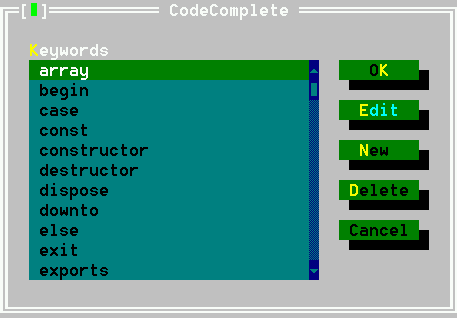
\epsfig{file=pics/ide/codecomp.png,width=\textwidth}
\else
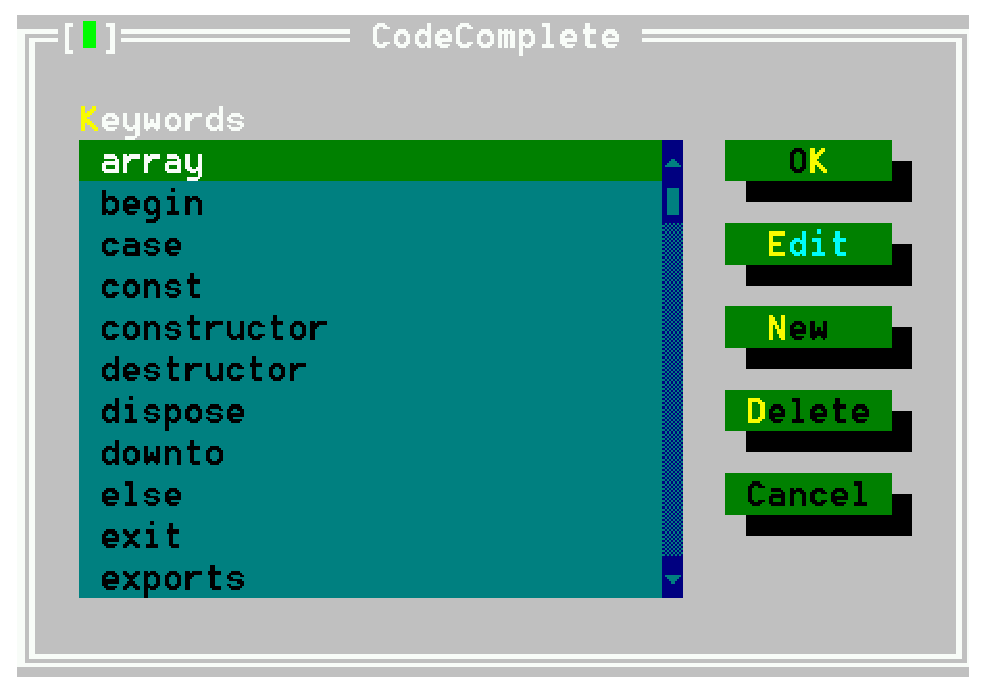
\epsfig{file=pics/ide/codecomp.eps,width=\textwidth}
\fi
\end{figure}
\end{latexonly}
The dialog shows the currently defined keywords that will be completed in
alphabetical order.
The following buttons are available:
\begin{description}
\item[Ok] Saves all changes and closes the dialog.
\item[Edit] Pops up a dialog that allows to edit the currently 
highlighted keyword.
\item[New] Pops up a dialog that allows to enter a new keyword which will be
added to the list.
\item[Delete] Deletes the currently highlighted keyword from the list
\item[Cancel] Discards all changes and closes the dialog.
\end{description}
All keywords are saved and are available the next time the IDE is started.
Duplicate names are not allowed. If an attempt is made to add a duplicate
name to the list, an error will follow.

% Code templates
\subsection{Code Templates}
Code templates are a way to insert large pieces of code at once. Each 
code templates is identified by a unique name. This name can be used to
insert the associated piece of code in the text.

For example, the name \var{ifthen} could be associated to the following
piece of code:
\begin{verbatim}
If Then
  begin
  end
\end{verbatim}
A code template can be inserted by typing its name, and pressing \key{Ctrl-J}
when the cursor is positioned right after the template name.

Code templates can be added and edited in the code templates dialog, reachable via
the menu option \menu{Options|\-Preferences|\-Codetemplates}. 

\begin{htmlonly}
The code templates dialog.
\htmladdimg{../pics/ide/codetemp.png}
\end{htmlonly}
\begin{latexonly}
The code templates dialog is shown in \seefig{codetemp}.
\begin{figure}[ht]
\caption{The code completion dialog.}\label{fig:codetemp}
\ifpdf
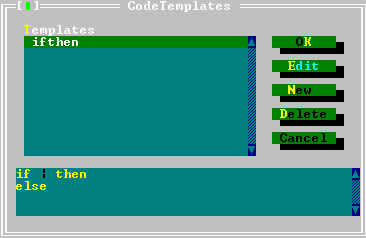
\epsfig{file=pics/ide/codetemp.png,width=\textwidth}
\else
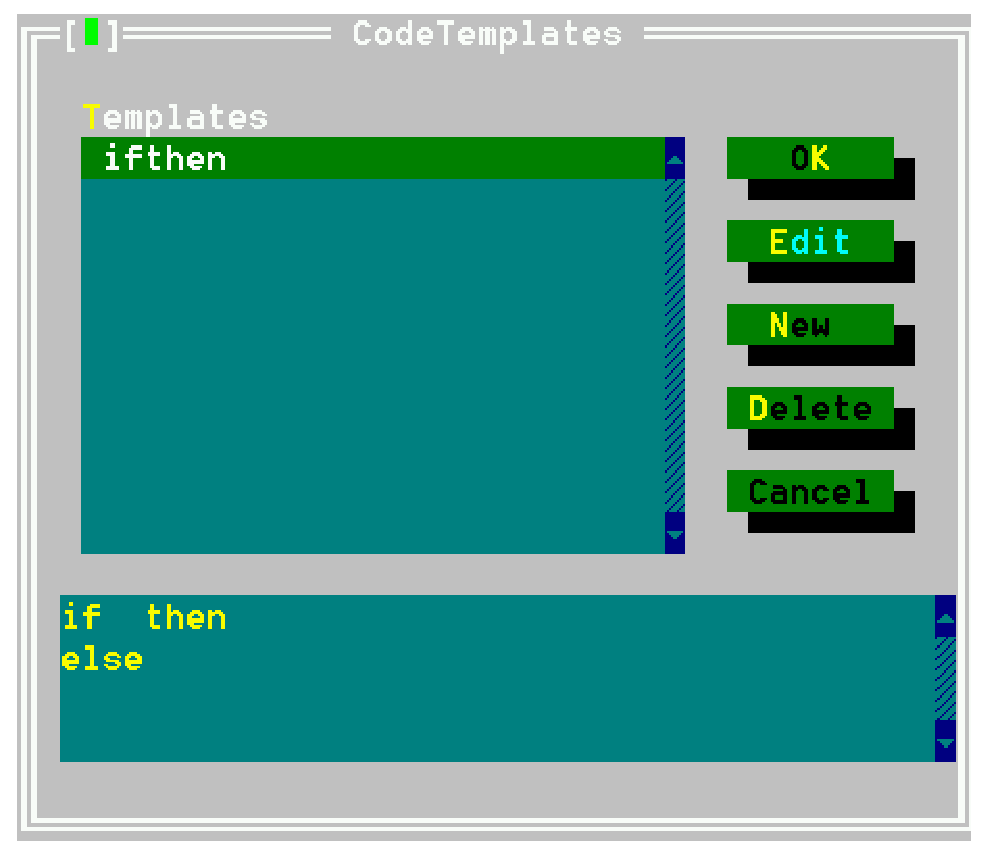
\epsfig{file=pics/ide/codetemp.eps,width=\textwidth}
\fi
\end{figure}
\end{latexonly}
The top listbox in the code templates dialog shows the names of all 
known templates. The bottom half of the dialog shows the text associated
with the currently highlighted code template.
The following buttons are available:
\begin{description}
\item[Ok] Saves all changes and closes the dialog.
\item[Edit] Pops up a dialog that allows to edit the currently 
highlighted code template. Both the name and text can be edited.
\item[New] Pops up a dialog that allows to enter a new code template
which will be added to the list. A name must be entered for the new
template.
\item[Delete] Deletes the currently highlighted code template from the list
\item[Cancel] Discards all changes and closes the dialog.
\end{description}
All templates are saved and are available the next time the IDE is started.
\begin{remark}
Duplicates are not allowed. If an attempt is made to add a duplicate name
to the list, an error will follow.
\end{remark}

%%%%%%%%%%%%%%%%%%%%%%%%%%%%%%%%%%%%%%%%%%%%%%%%%%%%%%%%%%%%%%%%%%%%%%%
% Searching in the text
\section{Searching and replacing}
\label{se:searching}
The IDE allows to search for text in the active editor window. 
To search for text, one  of the following can be done:
\begin{enumerate}
\item Select \menu{Search|Find} in the menu.
\item Press \key{Ctrl-Q F}.
\end{enumerate}
\begin{htmlonly}
After that, the following dialog will pop up:
\htmladdimg{../pics/ide/codetemp.png}
In this dialog, the following options can be entered:
\end{htmlonly}
\begin{latexonly}
After that, the dialog shown in \seefig{search} will pop up,
and the following options can be entered
\begin{figure}[ht]
\caption{The search dialog.}\label{fig:search}
\ifpdf
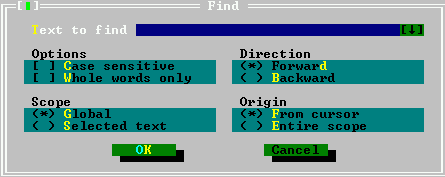
\epsfig{file=pics/ide/search.png,width=\textwidth}
\else
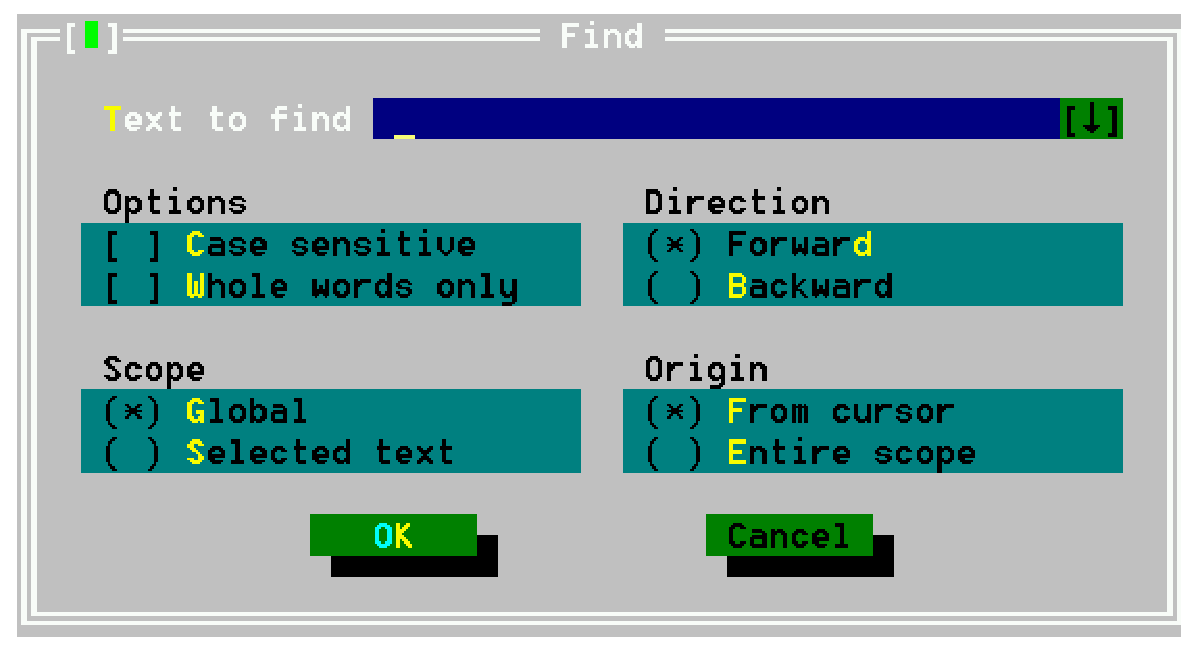
\epsfig{file=pics/ide/search.eps,width=\textwidth}
\fi
\end{figure}
\end{latexonly}

\begin{description}
\item[Text to find] The text to be searched for. If a block was active when
the dialog was started, this is proposed.
\item[Case sensitive] When checked, the search is case sensitive.
\item[Whole words only] When checked, the search text must appear in the
text as a complete word.
\item[Direction] The direction in which the search must be conducted,
starting from the specified origin.
\item[Scope] Should the search be on the whole file, or just the selected
text.
\item[Origin] Should the search start from the cursor position or the start
of the scope.
\end{description}
After the dialog is closed, the search is performed using the given options.

A search can be repeated (using the same options) in one of 2 ways:
\begin{enumerate}
\item Select \menu{Search|Find again} from the menu.
\item Press \key{Ctrl-L}.
\end{enumerate}

It is also possible to replace occurences of a text with another text. 
This can be done in a similar manner to searching for a text:
\begin{enumerate}
\item Select \menu{Search|Replace} from the menu.
\item Press \key{Ctrl-Q A}.
\end{enumerate}
A dialog, similar to the search dialog will pop up:
\begin{htmlonly}
A dialog, similar to the search dialog will pop up:
\htmladdimg{../pics/ide/codetemp.png}
In this dialog, the following options can be entered:
\end{htmlonly}
\begin{latexonly}
A dialog, similar to the search dialog will pop up, as shown in \seefig{replace}.
\begin{figure}[ht]
\caption{The replace dialog.}\label{fig:replace}
\ifpdf
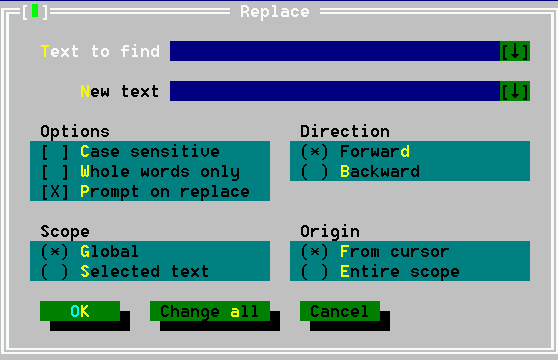
\epsfig{file=pics/ide/replace.png,width=\textwidth}
\else
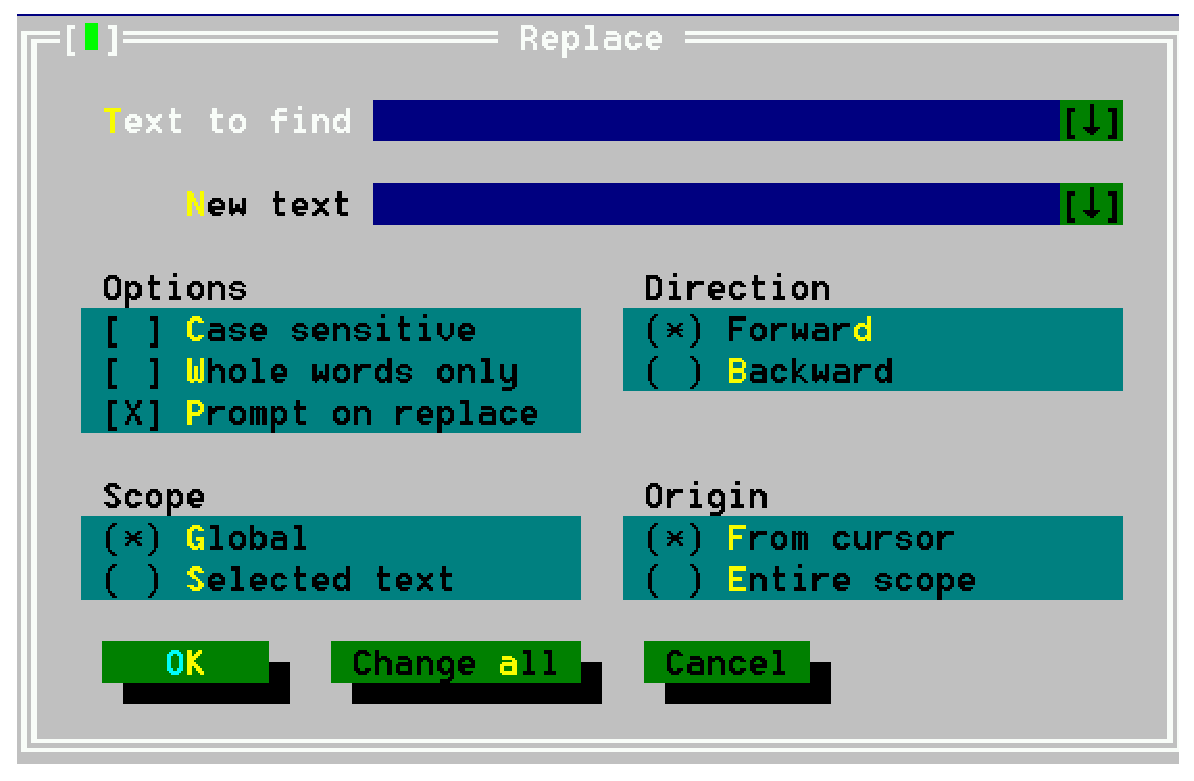
\epsfig{file=pics/ide/replace.eps,width=\textwidth}
\fi
\end{figure}
\end{latexonly}

In this dialog, in addition to the things that can be filled in in the
search dialog, the following things can be entered:
\begin{description}
\item [New text] Text by which found text will be replaced.
\item [Prompt on replace] Before a replacement is made, the IDE will ask for
confirmation.
\end{description}
If the dialog is closed with the 'OK' button, only the next occurrence of
the the search text will be replaced. 
If the dialog is closed with the 'Change All' button, all occurrences of 
the search text will be replaced.

%%%%%%%%%%%%%%%%%%%%%%%%%%%%%%%%%%%%%%%%%%%%%%%%%%%%%%%%%%%%%%%%%%%%%%%
% The symbol browser
\section{The symbol browser}
\label{se:browser}
The symbol browser allows to find all occurrences of a symbol. A symbol 
can be a variable, type, procedure or constant that occurs in your program.

To enable the symbol browser, the program or unit must be compiled with
browser information. This can be done by setting the browser information
option in the compiler options dialog.

The IDE allows to browse several types of symbols:
\begin{description}
\item[procedures] Allows to quickly jump to a procedure definition or
implementation.
\item[Objects] Allows to quickly browse an object.
\item[Modules] Allows to browse a module.
\item[Globals] Allows to browse any global symbol.
\item[Arbitrary symbol] Allows to browse an arbitrary symbol.
\end{description}
In all cases, first a symbol to be browsed must be selected. After that,
a browse window appears. In the browse window, all locations where the 
symbol was encountered are shown. Selecting a location and pressing the
space bar will cause the editor to jump to that location; the line
containing the symbol will be highlighted. 

If the location is in a source file that is not yet displayed, a new 
window will be opened with the source file loaded.

After the desired location was reached, the browse window can be closed 
with the usual commands. 

%%%%%%%%%%%%%%%%%%%%%%%%%%%%%%%%%%%%%%%%%%%%%%%%%%%%%%%%%%%%%%%%%%%%%%%
% Running programs
\section{Running programs}
\label{se:running}
A compiled program can be run straight from the IDE. This can be done
in one of several ways:
\begin{enumerate}
\item select the \menu{Run|Run} menu, or
\item press \key{Ctrl-F9}.
\end{enumerate}
If command-line parameters should be passed to the program, then these
can be set through the \menu{Run|Parameters} menu. 
\begin{htmlonly}
The Parameters dialog.
\htmladdimg{../pics/ide/params.png}
\end{htmlonly}
\begin{latexonly}
\begin{figure}[ht]
\caption{The program parameters dialog.}\label{fig:params}
\ifpdf
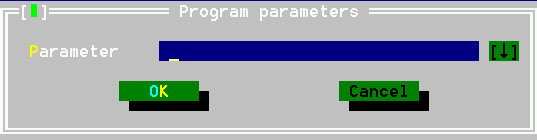
\epsfig{file=pics/ide/params.png,width=\textwidth}
\else
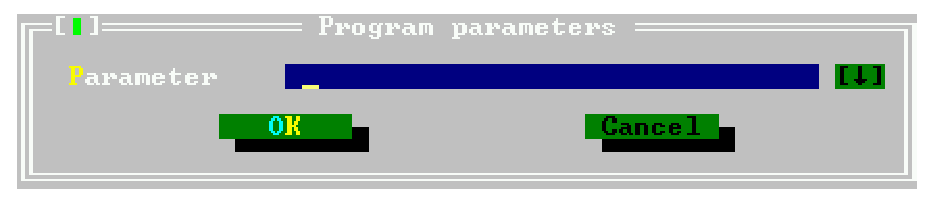
\epsfig{file=pics/ide/params.eps,width=\textwidth}
\fi
\end{figure}
\end{latexonly}

Once the program started, it will continue to run, until 
\begin{enumerate}
\item the program quits normally,
\item an error happens,
\item a breakpoint is encountered or
\item the program is reset by the user.
\end{enumerate}
The last alternative is only possible if the program is compiled
with debug information.

Alternatively, it is possible to position the cursor somewhere in a
source file, and run the program till the execution reaches the
source-line where the cursor is located. This can be done by
\begin{enumerate}
\item selecting \menu{Run|Goto Cursor} in the menu,
\item pressing \key{F4}.
\end{enumerate}
Again, this is only possible if the program was compiled with debug
information.

The program can also executed line by line. Pressing \key{F8} will 
execute the next line of the program. If the program wasn't started
yet, it is started. Repeatedly pressing \key{F8} will execute line 
by line of the program, and the IDE will show the line to be executed 
in an editor window. If somewhere in the code a call occurs to a subroutine,
then pressing \key{F8} will cause the whole routine to be executed before
control returns to the IDE. If the code of the subroutine should be stepped
through as well, then \key{F7} should be used instead. Using \key{F7} will
cause the IDE to execute line by line of any subroutine that is encountered.

If a subroutine is being stepped through, then the \menu{Run|Until return} menu
will execute the program till the current subroutine ends. 

If the program should be stopped before it quits by itself, then this can be
done by
\begin{enumerate}
\item selecting \menu{Run|Program reset} from the menu, or
\item pressing \key{Ctrl-F2}.
\end{enumerate}
The running program will then be aborted.

%%%%%%%%%%%%%%%%%%%%%%%%%%%%%%%%%%%%%%%%%%%%%%%%%%%%%%%%%%%%%%%%%%%%%%%
% Debugging programs
\section{Debugging programs}
\label{se:debugging}
To debug a program, it must be compiled with debug information. Compiling a
program with debug information allows to:
\begin{enumerate}
\item Execute the program line by line.
\item Run the program till a certain point (a breakpoint)
\item Inspect the contents of variables or memory locations while the
program is running.
\end{enumerate}
%
% Using breakpoints
%
\subsection{Using breakpoints}
Breakpoints will cause a running program to stop when the execution
reaches the line where the breakpoint was set. At that moment, control
is returned to the IDE, and it is possible to continue execution.

To set a breakpoint on the current source line, use the 
\menu{Debug|BreakPoint} menu entry, or press \key{Ctrl-F8}.

A list of current breakpoints can be obtained through the
\menu{Debu|Breakpoint list} menu. 
\begin{htmlonly}
The breakpoint list window looks as follows:
\htmladdimg{../pics/ide/brklist.png}
\end{htmlonly}
\begin{latexonly}
The breakpoint list window is shown in \seefig{brklist}
\begin{figure}[ht]
\caption{The breakpoint list window.}\label{fig:brklist}
\ifpdf
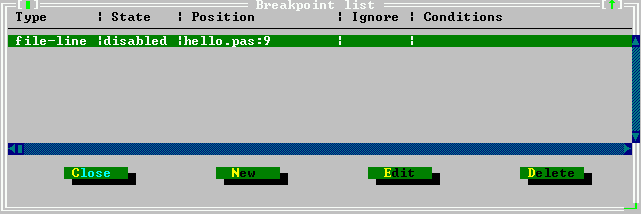
\epsfig{file=pics/ide/brklist.png,width=\textwidth}
\else
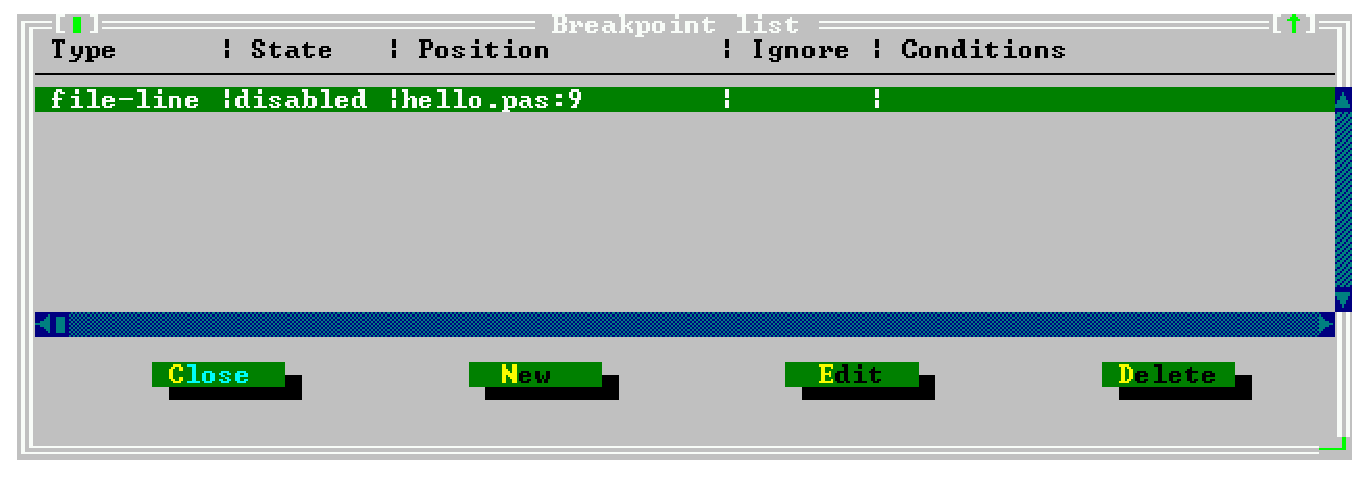
\epsfig{file=pics/ide/brklist.eps,width=\textwidth}
\fi
\end{figure}
\end{latexonly}
In the breakpoint list window, the following things can be done:
\begin{description}
\item[New] Shows the breakpoint property dialog where the properties
for a new breakpoint can be entered. 
\item[Edit] Shows the breakpoint property dialog where the properties of
the highlighted breakpoint can be changed. 
\item[Delete] Deletes the highlighted breakpoint.
\end{description}
The dialog can be closed with the 'Close' button.

\begin{htmlonly}
The breakpoint properties dialog looks as follows:
\htmladdimg{../pics/ide/brkprop.png}
\end{htmlonly}
\begin{latexonly}
The breakpoint properties dialog is shown in \seefig{brkprop}
\begin{figure}[ht]
\caption{The breakpoint properties dialog.}\label{fig:brkprop}
\ifpdf
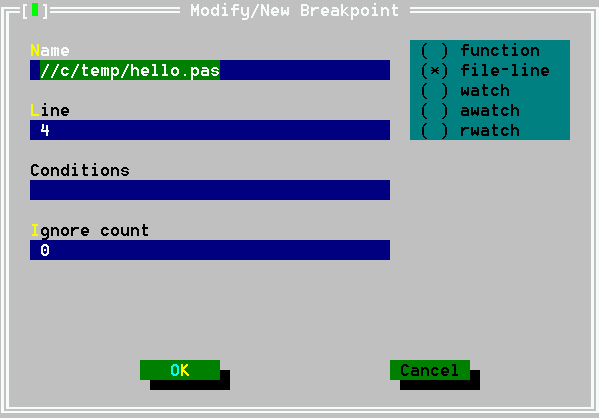
\epsfig{file=pics/ide/brkprop.png,width=\textwidth}
\else
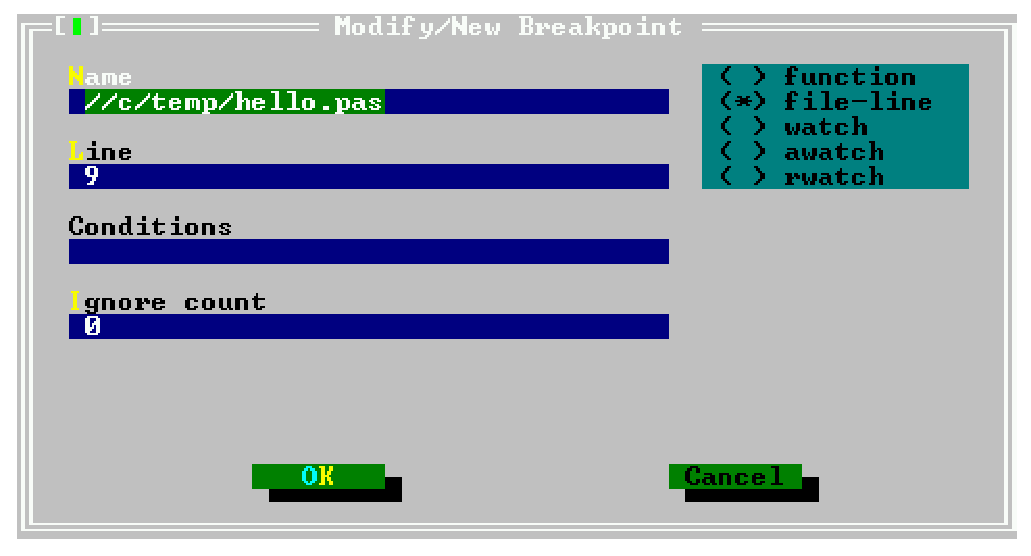
\epsfig{file=pics/ide/brkprop.eps,width=\textwidth}
\fi
\end{figure}
\end{latexonly}
The following properties can be set:
\begin{description}
\item[type]
\begin{description}
\item[function] function breakpoint. The program will stop when the function
with the given name is reached.
\item[file-line] Source line breakpoint. The program will stop when the
source file with given name and line is reached;
\item[watch] Expression breakpoint. An expression may be entered, and the
program will stop as soon as the expression changes.
\item[awatch] (access watch) Expression breakpoint. An expression that references a 
memory location may be entered, and the program will stop as soon as 
the memory indicated by the expression is accessed.
\item[rwatch] (read watch) Expression breakpoint. An expression that references a
memory location may be entered, and the program will stop as soon as 
the memory indicated by the expression is read.
\end{description}
\item[name] Name of the function or file where to stop.
\item[line] Line number in the file where to stop. Only for breakpoints of
type file-line.
\item[Conditions] Here an expression can be entered which must evaluate 
\var{True} for the program to stop at the breakpoint. The expressions that
can be entered must be valid GDB expressions.
\item[Ignore count] The number of times the breakpoint will be ignored
before the program stops; 
\end{description}
\begin{remark}
\begin{enumerate}
\item Because the IDE uses GDB to do its debugging, it is necessary to enter all
expressions in {\em uppercase} on \freebsd. 
\item Expressions that reference memory locations should be no longer than 16 
bytes on linux or go32v2 on an Intel processor, since the Intel processor's 
debug registers are used to monitor these locations.
\item Memory location watches will not function on Win32 unless a special 
patch is applied. 
\end{enumerate}
\end{remark}

%
% Using watches
%
\subsection{Using watches}
When debugging information is compiled in the program, watches can be used.
Watches are expressions which can be evaluated by the IDE and shown in a
separate window. When program execution stops (e.g. at a breakpoint) all
watches will be evaluated and their current values will be shown.

Setting a new watch can be done with the \menu{Debug|Add watch} menu 
command or by pressing \key{Ctrl-F7}. When this is done, the watch
property dialog appears, and a new expression can be entered.
\begin{htmlonly}
The watch property dialog looks as follows:
\htmladdimg{../pics/ide/watch.png}
\end{htmlonly}
\begin{latexonly}
The watch property dialog is shown in \seefig{brklist}
\begin{figure}[ht]
\caption{The watch property dialog.}\label{fig:watch}
\ifpdf
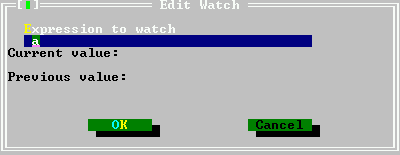
\epsfig{file=pics/ide/watch.png,width=\textwidth}
\else
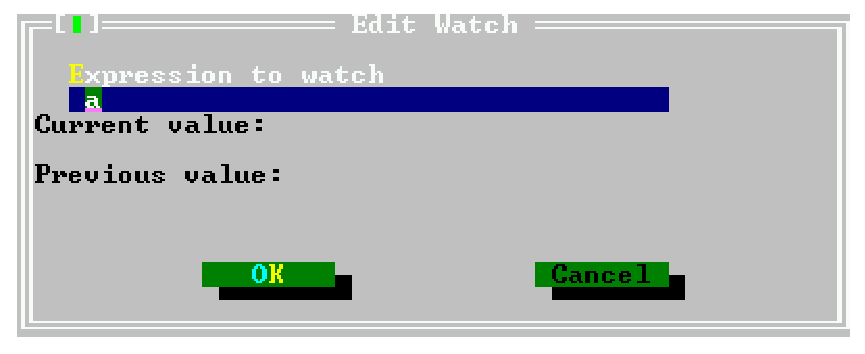
\epsfig{file=pics/ide/watch.eps,width=\textwidth}
\fi
\end{figure}
\end{latexonly}
In the dialog, the expression can be entered, any possible previous value
and current value are shown.
\begin{remark}
Because the IDE uses GDB to do it's debugging, it is necessary to enter all
expressions in {\em uppercase} in \freebsd. 
\end{remark}
A list of watches and their present value is available in the watches
window, which can be opened with the \menu{Debug|Watches} menu.
\begin{htmlonly}
The watch list window looks as follows:
\htmladdimg{../pics/ide/watch.png}
\end{htmlonly}
\begin{latexonly}
The watch list window is shown in \seefig{brklist}
\begin{figure}[ht]
\caption{The watch list window.}\label{fig:watchlst}
\ifpdf
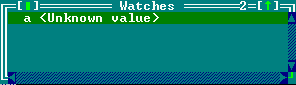
\epsfig{file=pics/ide/watchlst.png,width=\textwidth}
\else
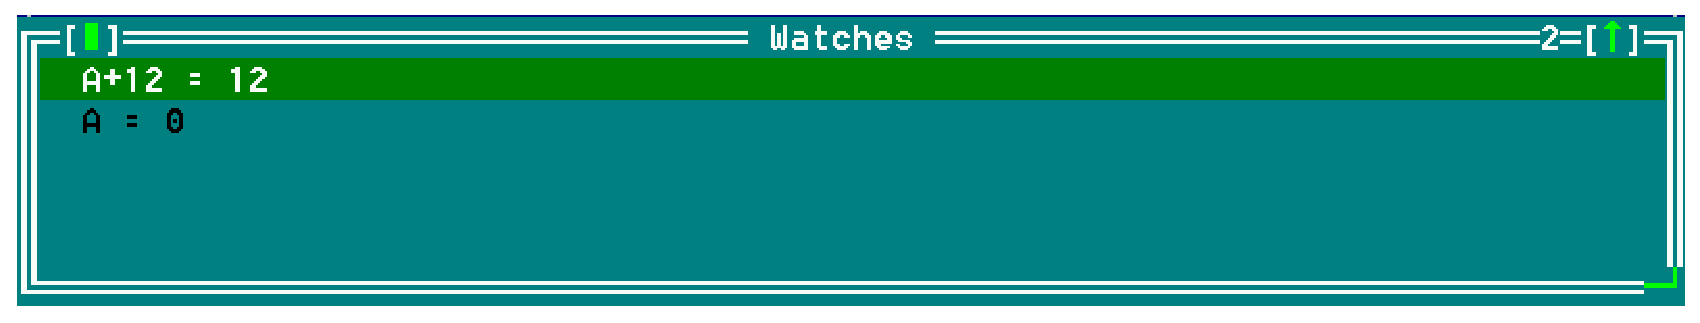
\epsfig{file=pics/ide/watchlst.eps,width=\textwidth}
\fi
\end{figure}
\end{latexonly}

Pressing \key{Enter} or the space bar will show the watch property dialog
for the currently highlighted watch in the watches window.

The list of watches is updated whenever the IDE resumes control when
debugging a program.
%
% The call stack
%
\subsection{The call stack}
\label{se:callstack}
The call stack helps in showing the program flow. It shows the list of
procedures that are being called at this moment, in reverse order.
The call stack window can be shown using the \menu{Debug|Call Stack}
It will show the address or procedure name of all currently active 
procedures with their filename and addresses. If parameters were passed
they will be shown as well.
\begin{htmlonly}

The call stack window looks as follows:
\htmladdimg{../pics/ide/watch.png}
\end{htmlonly}
\begin{latexonly}
The call stack is shown in \seefig{callstack}.
\begin{figure}[ht]
\caption{The call stack window.}\label{fig:callstack}
\ifpdf
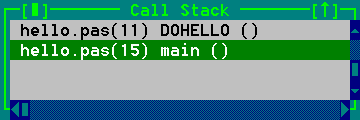
\epsfig{file=pics/ide/callstck.png}
\else
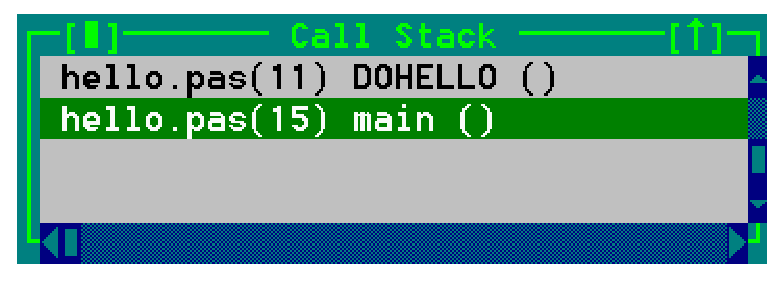
\epsfig{file=pics/ide/callstck.eps}
\fi
\end{figure}
\end{latexonly}

By pressing the space bar in the call stack window, the line curresponding
to the call will be highlighted in the edit window.

% The GDB Window
\subsection{The GDB window}
\label{se:gdbwindow}
The GDB window provides direct interaction with the GDB debugger.
In it, GDB commands can be typed as they would be typed in GDB.
The response of GDB will be shown in the window.

Some more information on using GDB can be found in \sees{usinggdb}, but
the final reference is of course the GDB manual itself
\footnote{Available from the free Software Foundation website.}.

\begin{htmlonly}
The GDB window looks as follows:
\htmladdimg{../pics/ide/gdbwin.png}
\end{htmlonly}
\begin{latexonly}
The GDB window is shown in \seefig{gdbwin}.
\begin{figure}[ht]
\caption{The GDB window.}\label{fig:gdbwin}
\ifpdf
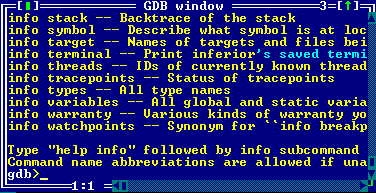
\epsfig{file=pics/ide/gdbwin.png,width=\textwidth}
\else
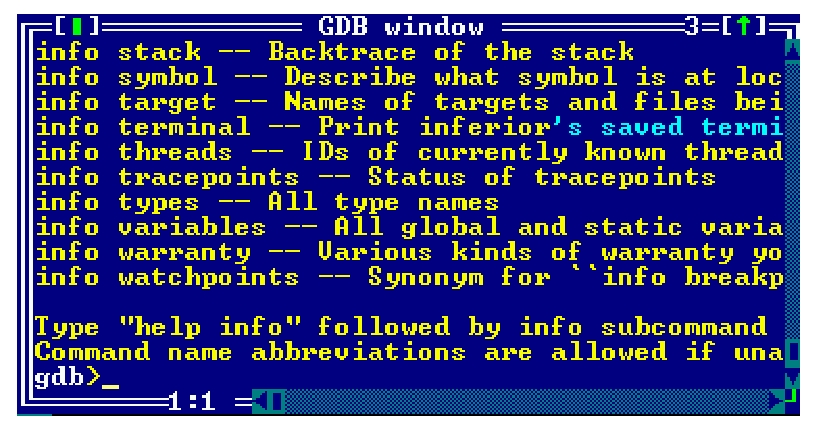
\epsfig{file=pics/ide/gdbwin.eps,width=\textwidth}
\fi
\end{figure}
\end{latexonly}

%%%%%%%%%%%%%%%%%%%%%%%%%%%%%%%%%%%%%%%%%%%%%%%%%%%%%%%%%%%%%%%%%%%%%%%
% The tools menu
\section{The Tools menu}
\label{se:toolsmenu}
The tools menu provides easy access to external tools. It also has
three pre-defined tools for programmers: an ASCII table,  a grep tool
and a calculator. The output of the external tools can be accessed through
this menu as well.

%
% The messages window.
%
\subsection{The messages window}
\label{se:toolsmessages}
The output of the external utilies is redirected by the IDE and it
will be displayed in the messages window. The messages window is
displayed automatically, if an external tool was run. The
messages window can be also displayed manually by the selecting the
menu item \menu{Tools|Messages} or by pressing the key \key{F11}.

\begin{htmlonly}
The messages window looks as follows:
\htmladdimg{../pics/ide/messages.png}
\end{htmlonly}
\begin{latexonly}
The messages window is shown in \seefig{messages}.
\begin{figure}[ht]
\caption{The messages window.}\label{fig:messages}
\ifpdf
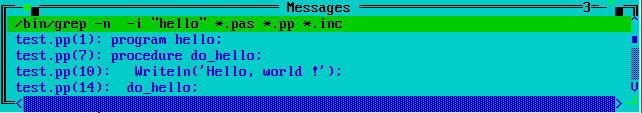
\epsfig{file=pics/ide/messages.png,width=\textwidth}
\else
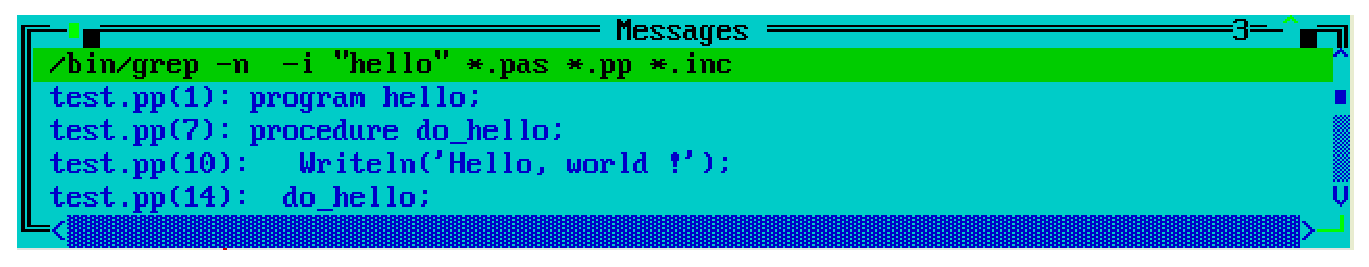
\epsfig{file=pics/ide/messages.eps,width=\textwidth}
\fi
\end{figure}
\end{latexonly}
If the output of the tool contains filenames and line numbers,
the messages window can be used to navigate the source as in a browse
window:
\begin{enumerate}
\item Pressing \key{Enter} or double clicking the output line will jump
to the specified source line and close the messages window.
\item Pressing the space bar will jump to the specified source line, but
will leave the messages window open, with the focus on it. This allows to
quickly select another message line with the arrow keys and jump to 
another location in the sources.
\end{enumerate}
The algorithm which extracts the file names and line numbers from
the tool output is quite sophisticated, but in some cases it may
fail\footnote{Suggestions for improvement, or better yet, patches
that improve the algorithm, are always welcome.}.
%
% Grep
%
\subsection{Grep}
\label{se:grep}
One external tool in the Tools menu is already predefined: a
menu item to call the \file{grep} utility (\menu{Tools|Grep} or
\key{Shift-F2}). \file{Grep} searches for a given string in files and
returns the lines which contain the string. The search string can
be even a regular expression. For this menu item to work, the
\file{grep} program must be installed, since it does not come with \fpc.

The messages window displayed in \seefig{messages} in the previous 
section shows the output of a typical \file{grep} session. The messages
window can be used in combination with \file{grep} to find special
occurrences in the text.

\file{Grep} supports regular expressions. A regular expression is a 
string with sepcial characters which describe a whole class of 
expressions. The command line in \dos or \linux have limited 
support for regular expressions: entering \var{ls *.pas} 
(or \var{dir *.pas}) to get a list of all pascal files in a
directory. \file{*.pas} is something similiar to regular expression. 
It uses a wildcard to describe a whole class of strings: these which 
end with "\file{.pas}". 
Regular expressions offer much more: for example \var{[A-Z][0-9]+} 
describes all strings which begin with a upper case letter followed by
one or more digits.

It is outside the scope of this manual to describe regular expressions
in great detail. Users of a \linux system can get more information on grep
using \var{man grep} on the command-line.
%
% The ascii table.
%
\subsection{The ASCII table}
\label{se:asciitable}
The tools menu provides also an ASCII table (\menu{Tools|Ascii table}),
The ascii table can be used to look up ASCII codes as well as
inserting characters into the window which was active when invoking the
table. To get the ASCII code of a char move the cursor on this char 
or click with the mouse on it. To insert a
char into an editor window either:
\begin{enumerate}
\item using the mouse, double click it,
\item using the keyboard,  press \key{Enter} while the cursor is on it.
\end{enumerate}
This is especially useful for pasting graphical characters in a constant
string.

The ASCII table remains active till another window is explicitly activated,
thus mulptiple characters can be inserted at once.
\begin{htmlonly}
The ASCII table looks as follows:
\htmladdimg{../pics/ide/ascii.png}
\end{htmlonly}
\begin{latexonly}
The ASCII table is shown in \seefig{asciitable}.
\begin{figure}[ht]
\caption{The ASCII table.}\label{fig:asciitable}
\ifpdf
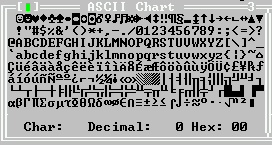
\epsfig{file=pics/ide/ascii.png}
\else
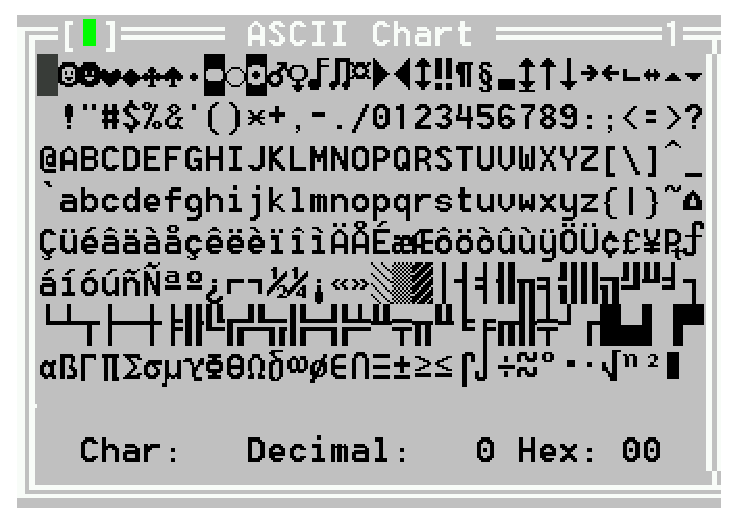
\epsfig{file=pics/ide/ascii.eps}
\fi
\end{figure}
\end{latexonly}

%
% The calculator
%
\subsection{The calculator}
\label{se:calculator}
The calculator allows to do some quick calculations. It is a simple
calculator, since it does not take care of operator precedence, and
bracketing of operations is not (yet) supported.

The result of the calculations can not yet be
pasted into the text, hopefully some future version of the IDE will support
pasting the result into the text.

\begin{htmlonly}
The calculator dialog looks as follows:
\htmladdimg{../pics/ide/calc.png}
\end{htmlonly}
\begin{latexonly}
The calculator dialog is shown in \seefig{calculator}.
\begin{figure}[ht]
\caption{The calculator dialog.}\label{fig:calculator}
\ifpdf
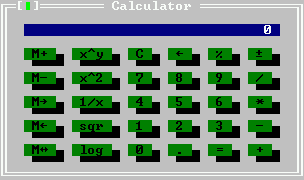
\epsfig{file=pics/ide/calc.png}
\else
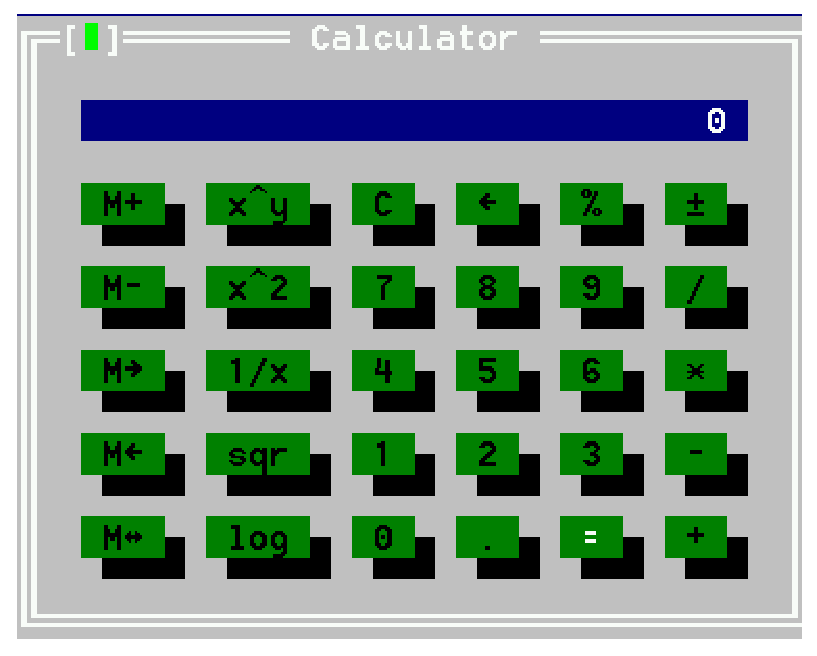
\epsfig{file=pics/ide/calc.eps}
\fi
\end{figure}
\end{latexonly}
The calculator supports all basic mathematical operations such as
addition, substraction, division and multiplication. They are summarized in
\seet{calculatorbasic}.
\begin{FPCltable}{p{8cm}lll}{Advanced calculator commands}{calculatorbasic}
Operation & Button & Key \\ \hline
Add two numbers & \var{+} & \key{+} \\
Subtract two numbers & \var{\-} & \key{\-} \\
Multiply two numbers & \var{*} & \key{*} \\
Divide two numbers & \var{/} & \key{/} \\
Delete the last typed digit & \var{<-} & \key{Backspace} \\
Delete the display & \var{C} & \key{C} \\
Change the sign & \var{+\-} & \\
Do per cent calculation & \var{\%} & \key{\%} \\ \hline
Get result of operation & \var{=} & \key{Enter} \\ \hline
\end{FPCltable}

But also more sophisticated mathematical operations such as exponentiation
and logarithms are supported. The available mathematical calculations are
shown in \seet{calculatoradvanced}.
\begin{FPCltable}{p{8cm}lll}{Advanced calculator commands}{calculatoradvanced}
Operation & Button & Key \\ \hline
Calculate power & \var{x\^y} & \\
Calculate the reciproke value & \var{1/x} & \\
Calculate the square root & \var{sqr} & \\
Calulate the natural logarithm &  \var{log} & \\
Square the display contents & \var{x\^2} & \\ \hline.
\end{FPCltable}

Like many calculators, the calculator in the IDE also supports storing
a single value in memory, and several operations can be done on this memory
value. The available operations are listed in \seet{calculatormemory}
\begin{FPCltable}{p{8cm}lll}{Advanced calculator commands}{calculatormemory}
Operation & Button & Key \\ \hline
Add the displayed number to the memory & \var{M+} & \\
Subtract the displayed number from the memory & \var{M-} & \\
Move the memory contents to the display & \var{M->} & \\
Move the display contents to the memory & \var{M<-} & \\
Exchange display and memory contents & \var{M<->} & \\ \hline
\end{FPCltable}
%
% Adding new tools
%
\subsection{Adding new tools}
\label{se:addingtools}
The tools menu can be extended with any external program which is command-line
oriented. The output of such a program will be caught and displayed in the 
messages window.

Adding a tool to the tools menu can be done using the \menu{Options|Tools} menu.
This will display the tools dialog.
\begin{htmlonly}
The tools dialog looks as follows:
\htmladdimg{../pics/ide/otools.png}
\end{htmlonly}
\begin{latexonly}
The tools dialog is shown in \seefig{otools}.
\begin{figure}[ht]
\caption{The ASCII table.}\label{fig:otools}
\ifpdf
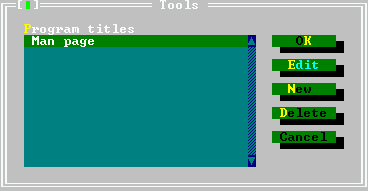
\epsfig{file=pics/ide/otools.png,width=\textwidth}
\else
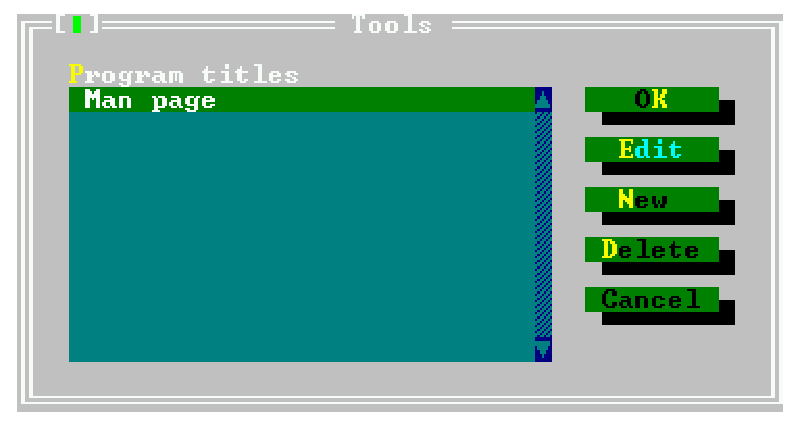
\epsfig{file=pics/ide/otools.eps,width=\textwidth}
\fi
\end{figure}
\end{latexonly}
In the tools dialog, the following actions are available:
\begin{description}
\item[New] Shows the tool properties dialog where the
properties of a new tool can be entered.
\item[Edit] Shows the tool properties dialog where the
properties of the highlighted tool can be edited.
\item[Delete] Removes the currently highlighted tool.
\item[Cancel] Discards all changes and closes the dialog.
\item[OK] Saves all changes and closes the dialog.
\end{description}
The definitions of the tools are written in the desktop
configuration file, so unless auto-saving of the desktop file
is enabled, the dektop file should be saved explicitly after
the dialog is closed.

\subsection{Meta parameters}
When specifing the command line for the called tool, meta parameters can
be used. Meta parameters are variables and and they are replaced
by their contents before passing the command line to the tool.

\begin{description}
\item[\$CAP] 
\item[\$CAP\_MSG]
Captures the output of the tool and puts it in the messages window.
\item[\$CAP\_EDIT]
Captures the output of the tool and puts it in a separate editor window.
\item[\$COL]
Replaced by the colomn of the cursor in the active editor window. If there is no
 active window or the active window is a dialog, then it is replaced by 0.
\item[\$CONFIG]
Replaced by the complete filename of the current configuration file.
\item[\$DIR()]
Replaced by the full directory of the filename argument, including trailing
directory separator. e.g.
\begin{verbatim}
  $DIR('d:\data\myfile.pas')
\end{verbatim}
would return \verb|d:\data\|.
\item[\$DRIVE()]
Replaced by the drive letter of the filename argument. e.g.
\begin{verbatim}
  $DRIVE('d:\data\myfile.pas')
\end{verbatim}
would return \file{d:}.
\item[\$EDNAME]
Replaced by the complete file name of the file in the active edit window.
If there is no active edit window, this is an empty string.
\item[\$EXENAME]
Replaced by the executable name that would be created if the make command
was used. (i.e. from the 'Primary File' setting or the active edit window).
\item[\$EXT()]
Replaced by the extension of the filename argument.
The extension includes the dot.
e.g.
\begin{verbatim}
  $DIR('d:\data\myfile.pas')
\end{verbatim}
would return \file{.pas}.
\item[\$LINE]
Replaced by the line number of the cursor in the active edit window.
If no edit window is present or active, this is 0.
\item[\$NAME()]
Replaced by the name part (excluding extension and dot) of the filename
argument.
e.g.
\begin{verbatim}
  $NAME('d:\data\myfile.pas')
\end{verbatim}
would return \file{myfile}.
\item[\$NAMEEXT()]
Replaced by the name and extension part of the filename argument.
e.g.
\begin{verbatim}
  $DIR('d:\data\myfile.pas')
\end{verbatim}
would return \file{myfile.pas}.
\item[\$NOSWAP]
Does nothing in the IDE, it is provided for compatibility with \tp only.
\item[\$PROMPT()]
Prompt displays a dialog bow that allows editing of all arguments that
come after it. Arguments that appear before the \var{\$PROMPT} keyword
are not presented for editing.

If a (optional) filename argument is present, \var{\$PROMPT()} will load
a dialog description from the filename argument, e.g.
\begin{verbatim}
$PROMPT('cvsco.tdf')
\end{verbatim}
would parse the file \file{cvsco.tdf}, construct a dialog with it and
display it. After the dialog closed, the information entered by the user
is used to construct the tool command line.

See \sees{commanddialogs} for more information on how to create a dialog
description.
\item[\$SAVE]
Befure executing the command, the active editor window is saved, even if it is not modified.
\item[\$SAVE\_ALL]
Before executing the command, all unsaved editor files are saved without prompting.
\item[\$SAVE\_CUR]
Before executing the command the contents of the active editor window are
saved without prompting if they are modified.
\item[\$SAVE\_PROMPT]
Before executing the command, a dialog is displayed askeing whether any
unsaved files should be saved before executing the command.
\item[\$WRITEMSG()]
Writes the parsed tool output information to a file with name as in the argument.
\end{description}	

\subsection{Building your own tool command line dialog box}
\label{se:commanddialogs}


%%%%%%%%%%%%%%%%%%%%%%%%%%%%%%%%%%%%%%%%%%%%%%%%%%%%%%%%%%%%%%%%%%%%%%%
% Project management
\section{Project management}
\label{se:projectmanagement}
Luckily, project mangament in pascal is much easier than with C. The
compiler knows from the source which units, sources etc. it needs.
So the \fpc IDE does not need a full featured project manager like
some C development environments offer. But some things make life easier...

\subsection{The primary file}
\label{se:primaryfile}
Without a primary file the IDE compiles/runs the source of the actived
window when you start your program. If you have specified a primary
file, the IDE compiles/runs always this source, no matter if another
source window is active. Select the menu item \var{Compile|Primary file...}
to get a file dialog where you can enter the primary file. Only the command
\var{Compile|Compile} compiles still the active window, this is usefull
if you have a large project and you want only check the syntax of the
current source.

The menu item \var{Compiler|Clear primary file} restores the default behavior
i.e. the compile and run commands apply to the active window.

\subsection{The switches mode}
\label{se:compilermode}
The IDE allows you to work with three different sets of compiler
switches: Normal, Debug and Release. The different switch
sets can be selected in the \var{Switches Mode} dialog which
is executed by the menu item \var{Options|Mode...}.
Change the switches mode doesn't do any active switch change, i.e.
the debug mode doesn't include debug information automatically,
it just loads another set of switches which were adjusted before
by the user in the compiler or directory dialog.

\subsection{The directory dialog}
In the directory dialog, you've to specify the directories where
the compiler should look for units, library etc, where the
output files should be stored etc. You can specify multiple
directories (except for the output directory) seperated by
semicolon.

\begin{description}
\item Nothing yet !!!!!!!!!!!!!!
\end{description}

\subsection{The target operating system}
The menu item \var{Compile|Target} allows you to specify the target
operating system. Changing the target doesn't affect any compiler
switches or directories.

\subsection{The configuration files}
%%%!!!!!!!!!!!!!!

%%%%%%%%%%%%%%%%%%%%%%%%%%%%%%%%%%%%%%%%%%%%%%%%%%%%%%%%%%%%%%%%%%%%%%%
% Customize the IDE
\section{Customize the IDE}
The IDE is configurable in a wide range, you can change colors, screen
resolution etc. The configuration setting can reached via the
submenu \var{Environment} in the \var{Options} menu.

\subsection{Preferences}
The \emph{preferences dialog} is called by the menu item
\var{Options|Environment|Preferences}.

%%%!!!!!!!!!!!!!!

\subsubsection{Video modes}
The \emph{drop down list} at the top of the dialog allows you
to select a video mode.

\begin{remark}
You have to select the video mode by pressing space or clicking
on it. If the drop down list is opened while leaving the dialog,
the new video mode will not be applied.
\end{remark}

The available video modes depend on the system on which the IDE
is running. 

\begin{remark}
If you're using VESA modes under DOS, the display refresh rate may be
annoying low. On older graphics card (1998 and before),
you can try to use the \emph{UniVBE} driver of \emph{SciTech}. But
it is quite outdated (last update somewhere in 1998). For newer
graphics cards which support VESA 3.0, you can try to get one
of the TSR programs
\footnote{\textbf{T}erminate and \textbf{S}tay \textbf{R}esisdent}
available at the net to customize the refresh rate.
%%%%!!!!!!!! footnote with URL
\end{remark}

\subsection{Mouse}
\label{se:prefmouse}
The \emph{mouse options dialog} is called by the menu item
\var{Options|Environment|Mouse}. You can use the slider to adjust the
double clock speed. If you're left handed you can exchange the
behavior of the left and right mouse button by checking the checkbox
item \var{Reverse mouse buttons}.

The two lists with the radio buttons allows you
to configure the behavior of the
right mouse button, if it is clicked together while
pressing the \key{Ctrl} or
\key{Alt} key in an edit window.

The following actions can be assigned to \key{Ctrl}-right mouse button or
\key{Alt}-right mouse button:

\begin{description}
\item [Topic search] The keyword at the mouse cursor is searched in the
help index
\item [Go to cursor] The program is executed until the line where
the mouse cursor is located
\item [Breakpoint] Set a breakpoint at the mouse cursor position
\item [Evalute] Evaluate the value of the variable at the mouse
cursor
\item [Add watch] Add the variable at the mouse cursor to the
watch window
\item [Browse symbol] The symbol at the mouse cursor is displayed
by the browser
\end{description}


%%%%%%%%%%%%%%%%%%%%%%%%%%%%%%%%%%%%%%%%%%%%%%%%%%%%%%%%%%%%%%%%%%%%%%%
% The help system
\section{The help system}

More information on how to handle the IDE, or about the use of various
calls in the RTL, explanations regarding the syntax of a pascal statement,
can be found in the \emph{help system}. The help system is activated
by pressing \key{F1}.

\subsection{Navigating in the help system}
The help system contains hyperlinks; these are sensitive locations that
lead to another topic in the help system. They are marked by a different
color. The hyperlinks can be activated in 2 ways:
\begin{enumerate}
\item by clicking them with the mouse,
\item by using the \key{Tab} and \key{Shift-Tab} keys to move between 
the different hyperlinks of a page and the \key{Enter} key can be used 
to activate them.
\end{enumerate}

The contents of the help system is displayed, if \key{Shift-F1} is
pressed. To go back to the previous help topic, press \key{Alt-F1}. 
This also works if the help window isn't displayed on the desktop; the help
window will then be activated.

%
% Working with help files.
%
\subsection{Working with help files}
The IDE contains a help system which can display the following file formats:
\begin{description}
\item[TPH] The help format for the Turbo Pascal help viewer.
\item[INF] The OS/2 help format.
\item[NG] The NGHelp format.
\item[HTML] HTML files. 
The HTML viewer of the  help system is limited, it can only handle the 
most basic HTML files not including graphics, since it is only designed 
to display the \fpc help files \footnote{...but feel free to improve it and send patches to the 
\fpc development team...}.
\end{description}
The menu item \menu{Help|Files} permits you to add and delete
help files.
\begin{htmlonly}
The Help files dialog looks as follows:
\htmladdimg{../pics/ide/helpfils.png}
\end{htmlonly}
\begin{latexonly}
The help files dialog is displayed in \seefig{helpfiles}.
\begin{figure}[ht]
\caption{The help files dialog.}\label{fig:helpfiles}
\ifpdf
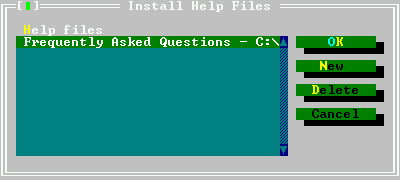
\epsfig{file=pics/ide/helpfils.png,width=\textwidth}
\else
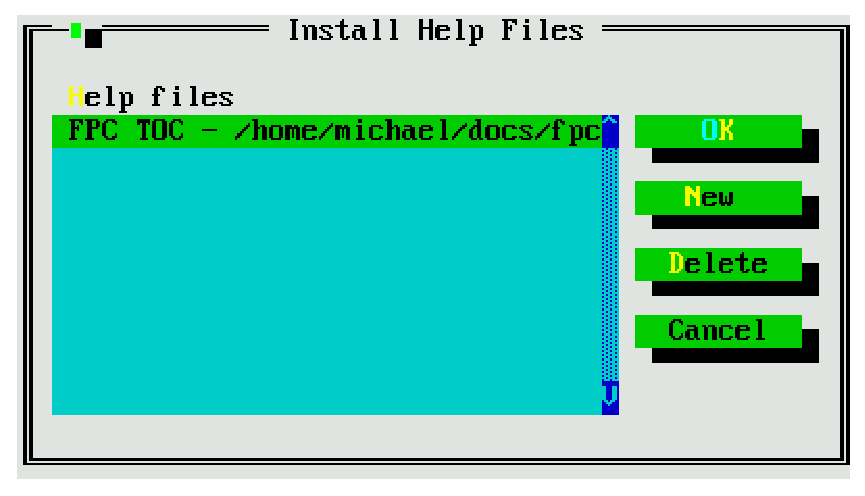
\epsfig{file=pics/ide/helpfils.eps,width=\textwidth}
\fi
\end{figure}
\end{latexonly}
The dialogs lists the files that will be presented in thetable of contents
window of the help system. Each entry has a small descriptive title and a
filename next to it. The following actions are available when adding help
files:
\begin{description}
\item[New] Adds a new file. IDE will display a prompt, in which the 
location of the help file should be entered. 

If the added file is an HTML file, a dialog box will be displayed
which asks for a title. This title will then be included in the
contents of help.
\item[Delete] Deletes the currently highlighted file from the help system.
It is \emph{not} deleted from the hard disk, only the help system entry is
removed.
\item[Cancel] Discards all changes and closes the dialog.
\item[OK] Saves the changes and closes the dialog.
\end{description}

The \fpc documentation in HTML format can be added to the IDE's help system,
this way the documentation can be viewed from within the IDE.

%
% The about dialog.
%
\subsection{The about dialog}
\label{se:about}
The \emph{about dialog} (\menu{Help|About...}) shows some information
about the IDE, such as the version number, the date it was built, what
compiler and debugger it uses. When reporting bugs about the IDE, please 
It also contains copyright information.


%%%%%%%%%%%%%%%%%%%%%%%%%%%%%%%%%%%%%%%%%%%%%%%%%%%%%%%%%%%%%%%%%%%%%%%
% Keyboard shortcuts
\section{Keyboard shortcuts}
\label{se:keyshortcuts}
A lot of keyboard shortcuts used by the IDE are compatible with 
WordStar and should be well known to Turbo Pascal users.

Below are the following tables:
\begin{enumerate}
\item In \seet{shortcutsgeneral} some shortcuts for handling the IDE windows
and Help are listed.
\item In \seet{shortcutscompiler} the shortcuts for compiling, running and
debugging a program are presented.
\item In \seet{shortcutsnavigation} the navigation keys are described.
\item In \seet{shortcutsedit} the editing keys are listed.
\item In \seet{shortcutsblock} lists all block command shortcuts.
\item In \seet{shortcutsselection} all selection-changing shortcuts are 
presented.
\item In \seet{shortcutsmisc} some general shortcuts are presented, 
which do not fit in the previous categories.
\end{enumerate}

\begin{FPCltable}{p{5cm}ll}{General}{shortcutsgeneral}
Command & Key shortcut & Alternative \\ \hline
Help & \key{F1} & \\
Goto last help topic & \key{Alt-F1} & \\
Search word at cursor position in help & \key{Ctrl-F1} & \\
Help index & \key{Shift-F1} & \\
Close active window & \key{Alt-F3} & \\
Zomm/Unzoom window & \key{F5} & \\
Move/Zoom active window & \key{Ctrl-F5} & \\
Switch to next window & \key{F6} & \\
Switch to last window & \key{Shift-F6} & \\
Menu & \key{F10} & \\
Local menu & \key{Alt-F10} & \\
List of windows & \key{Alt-0} & \\
Active another window & \key{Alt-<digit>} & \\
Call \file{grep} utility & \key{Shift-F2} & \\
Exit IDE & \key{Alt-X} & \\
\end{FPCltable}

%%%%%%%%%%%%%%%%%%%%%%%%%%%%%%%%%%%%%%%%%%%%%%%%%%%%%%%%%%%%%%%%%%%%%%%%%%%%
\begin{FPCltable}{p{5cm}ll}{Compiler}{shortcutscompiler}
Command & Key shortcut & Alternative \\
\hline
Reset debugger/program & \key{Ctrl-F2} & \\
Display call stack & \key{Ctrl-F3} & \\
Run til cursor & \key{F4} & \\
Switch to user screen & \key{Alt-F5} & \\
Trace into & \key{F7} & \\
Add watch & \key{Ctrl-F7} & \\
Step over & \key{F8} & \\
Set breakpoint at current line & \key{Ctrl-F8} & \\
Make & \key{F9} & \\
Run & \key{Ctrl-F9} & \\
Compile the active source file & \key{Alt-F9} & \\
Message & \key{F11} & \\
Compiler messages & \key{F12} & \\
\end{FPCltable}

%%%%%%%%%%%%%%%%%%%%%%%%%%%%%%%%%%%%%%%%%%%%%%%%%%%%%%%%%%%%%%%%%%%%%%%%%%%%
\begin{FPCltable}{p{5cm}ll}{Text navigation}{shortcutsnavigation}
Command & Key shortcut & Alternative \\
\hline
Char left & \key{Arrow left} & \key{Ctrl-S} \\
Char right & \key{Arrow right} & \key{Ctrl-D} \\
Line up & \key{Arrow up} & \key{Ctrl-E} \\
Line down & \key{Arrow down} & \key{Ctrl-X} \\
Word left & \key{Ctrl-Arrow left} & \key{Ctrl-A} \\
Word right & \key{Ctrl-Arror right} & \key{Ctrl-F} \\
Scroll one line up & \key{Ctrl-W} & \\
Scroll one line down & \key{Ctrl-Z} & \\
Page up & \key{PageUp} & \key{Ctrl-R} \\
Page down & \key{PageDown} & \\
Beginning of Line & \key{Pos1} & \key{Ctrl-Q-S} \\
End of Line & \key{End} & \key{Ctrl-Q-D} \\
First line of window & \key{Ctrl-Pos1} & \key{Ctrl-Q-E} \\
Last line of window & \key{Ctrl-End} & \key{Ctrl-Q-X} \\
First line of file & \key{Ctrl-PageUp} & \key{Ctrl-Q-R} \\
Last line of file & \key{Ctrl-PageDown} & \key{Ctrl-Q-C} \\
Last cursor position & \key{Ctrl-Q-P} & \\
\end{FPCltable}
%%%%%%%%%%%%%%%%%%%%%%%%%%%%%%%%%%%%%%%%%%%%%%%%%%%%%%%%%%%%%%%%%%%%%%%%%%%%
\begin{FPCltable}{p{5cm}ll}{Edit}{shortcutsedit}
Command & Key shortcut & Alternative \\
\hline
Delete char & \key{Del} & \key{Ctrl-G} \\
Delete left char & \key{Backspace} & \key{Ctrl-H} \\
Delete line & \key{Ctrl-Y} & \\
Delete til end of line & \key{Ctrl-Q-Y} & \\
Delete word & \key{Ctrl-T} & \\
Insert line & \key{Ctrl-N} & \\
Toggle insert mode & \key{Insert} & \key{Ctrl-V} \\
\end{FPCltable}

%%%%%%%%%%%%%%%%%%%%%%%%%%%%%%%%%%%%%%%%%%%%%%%%%%%%%%%%%%%%%%%%%%%%%%%%%%%%
\begin{FPCltable}{p{5cm}ll}{Block commands}{shortcutsblock}
Command & Key shortcut & Alternative \\
\hline
Goto Beginning of selected text & \key{Ctrl-Q-B} & \\
Goto end of selected text & \key{Ctrl-Q-K} & \\
Select current line & \key{Ctrl-K-L} & \\
Print selected text & \key{Ctrl-K-P} & \\
Select current word & \key{Ctrl-K-T} & \\
Delete selected text & \key{Ctrl-Del} & \key{Ctrl-K-Y} \\
Copy selected text to cursor position & \key{Ctrl-K-C} & \\
Move selected text to cursor position & \key{Ctrl-K-V} & \\
Copy selected text to clipboard & \key{Ctrl-Ins} & \\
Move selected text to the clipboard & \key{Shift-Del} & \\
Indent block one coloumn & \key{Ctrl-K-I} & \\
Unindent block one coloumn & \key{Ctrl-K-U} & \\
Insert text from clipboard & \key{Shift-Insert} & \\
Insert file & \key{Ctrl-K-R} & \\
Write selected text to file & \key{Ctrl-K-W} & \\
\end{FPCltable}

%%%%%%%%%%%%%%%%%%%%%%%%%%%%%%%%%%%%%%%%%%%%%%%%%%%%%%%%%%%%%%%%%%%%%%%%%%%%
\begin{FPCltable}{p{5cm}ll}{Change selection}{shortcutsselection}
Command & Key shortcut & Alternative \\
\hline
Mark beginning of selected text & \key{Ctrl-K-B} & \\
Mark end of selected text& \key{Ctrl-K-K} & \\
Remove selection & \key{Ctrl-K-Y} & \\
Extend selection one char to the left & \key{Shift-Arrow left} & \\
Extend selection one char to the right & \key{Shift-Arrow right} & \\
Extend selection to the beginning of the line & \key{Shift-Pos1} & \\
Extend selection to the end of the line & \key{Shift-End} & \\
Extend selection to the same coloumn in the last row & \key{Shift-Arrow up} & \\
Extend selection to the same coloumn in the next row & \key{Shift-Arrow down} & \\
Extend selection to the end of the line & \key{Shift-End} & \\
Extend selection one word to the left & \key{Ctrl-Shift-Arrow left} & \\
Extend selection one word to the right & \key{Ctrl-Shift-Arrow right} & \\
Extend selection one page up & \key{Shift-PageUp} & \\
Extend selection one page down & \key{Shift-PageDown} & \\
Extend selection to the beginning of the file & \key{Ctrl-Shift-Pos1} &
\key{Ctrl-Shift-PageUp} \\
Extend selection to the end of the file & \key{Ctrl-Shift-End} &
\key{Ctrl-Shift-PageUp} \\
\end{FPCltable}

%%%%%%%%%%%%%%%%%%%%%%%%%%%%%%%%%%%%%%%%%%%%%%%%%%%%%%%%%%%%%%%%%%%%%%%%%%%%
\begin{FPCltable}{p{5cm}ll}{Misc. commands}{shortcutsmisc}
Command & Key shortcut & Alternative \\
\hline
Save file & \key{F2} & \key{Ctrl-K-S} \\
Open file & \key{F3} & \\
Search & \key{Ctrl-Q-F} & \\
Search again & \key{Ctrl-L}\ & \\
Search and replace & \key{Ctrl-Q-A} & \\
Set mark & \key{Ctrl-K-n} (where n can be 0..9) & \\
Goto mark & \key{Ctrl-Q-n} (where n can be 0..9) & \\
Undo & \key{Alt-Backspace} & \\
\end{FPCltable}
%
%  $Log$
%  Revision 1.1.2.9  2000-11-21 14:16:06  michael
%  + Pages 1-23 corrected after remarks from Luk Vandelaer
%
%  Revision 1.1.2.8  2000/11/20 18:53:52  michael
%  + Documenting tools
%
%  Revision 1.1.2.7  2000/11/19 23:08:32  michael
%  + Further implementation.
%
%  Revision 1.1.2.6  2000/11/18 00:06:11  michael
%  + Added code templates
%  + Added syntax highlighting
%  + Added codecompletion
%  + Added gdb window
%
%  Revision 1.1.2.5  2000/11/15 23:43:32  michael
%  + Debugging finished
%
%  Revision 1.1.2.4  2000/11/15 18:58:35  michael
%  + Debug continued
%
%  Revision 1.1.2.3  2000/11/14 23:24:09  michael
%  + Documented run menu
%
%  Revision 1.1.2.2  2000/11/13 23:46:03  michael
%  + documented blocks, search, and the browser
%
%  Revision 1.1.2.1  2000/11/12 23:40:32  michael
%  + Changes for final version
%
%  Revision 1.1  2000/07/13 09:10:04  michael
%  + Initial import
%
%  Revision 1.5  2000/03/04 07:47:28  florian
%    * some corrections and some new stuff
%
%  Revision 1.4  2000/03/01 15:39:40  florian
%    * some new stuff
%
%  Revision 1.3  2000/02/28 17:45:40  florian
%    * a lot of new stuff
%